\documentclass[italian, a4paper, 12pt]{article}

\usepackage[utf8]{inputenc}
\usepackage[T1]{fontenc}
\usepackage{babel}

\usepackage[left=25mm, top=20mm, right=25mm, bottom=20mm]{geometry}
\renewcommand{\baselinestretch}{1.5}

\usepackage{float}

%%% font & looks %%%
\usepackage{mathpazo}
%\usepackage{palatino}
%\usepackage{kpfonts}
%\usepackage{times}
%\usepackage{charter}
%\usepackage{utopia}

% list of fonts available here - http://www.tug.dk/FontCatalogue/
% and here - https://www.sharelatex.com/learn/Font_typefaces

\usepackage{microtype}

\usepackage[parfill]{parskip}

\usepackage{bm}
\usepackage[labelfont=bf,font={small,it}]{caption}
\usepackage[usenames,dvipsnames,svgnames,table]{xcolor}

\usepackage{newtxtext}
\usepackage{newtxmath}

%%% boxes %%%
\usepackage{framed}
%\setlength\FrameSep{0.5em}

% math
%\usepackage{amsmath}
\usepackage{amssymb}
%\usepackage{amsthm}
\usepackage{wasysym}
%\usepackage{siunitx}

% graphics
\usepackage{multirow}
\usepackage[section]{placeins}
\usepackage{graphicx}
\usepackage{epstopdf}
\usepackage{pgfplots}
  \pgfplotsset{compat=newest}
  %% the following commands are needed for some matlab2tikz features
  \usetikzlibrary{plotmarks}
  \usetikzlibrary{arrows.meta}
  \usepgfplotslibrary{patchplots}
  \usepackage{grffile}
  \usepackage{amsmath}

\usepackage{pdfpages}

% extra
\usepackage{todonotes} %\todo{ note } , \listoftodos
\usepackage{blindtext}
\usepackage{lipsum}
\usepackage{tikz}
\usetikzlibrary{patterns}
\usetikzlibrary{decorations.pathreplacing,angles,quotes}
\usepackage{chemformula}
\usepackage{textcomp}
\usepackage{subcaption}

% better tables
\usepackage{booktabs}

%%% links %%%
\usepackage{hyperref}
\hypersetup{
        linktocpage,
        colorlinks,
    citecolor=black,
    filecolor=black,
    linkcolor=black,
    urlcolor=black
}

\usepackage[framed,numbered]{matlab-prettifier}
\tikzset{
  font={\fontsize{9pt}{12}\selectfont}}

\usepackage[sorting=none]{biblatex}
\addbibresource{report.bib}

%%% references %%%
\usepackage[noabbrev,capitalize,nameinlink]{cleveref}

% new commands
\newcommand{\horline}{\rule{1\linewidth}{0.9pt}}
\newcommand{\curl}{\nabla \times}
\renewcommand{\div}{\nabla \cdot}
\newcommand{\laplac}{\nabla^2}
\newcommand{\grad}{\nabla}

%\usepackage{mathspec}

%\newcommand{\mathbbm}[1]{\text{\usefont{U}{bbm}{m}{n}#1}} % from mathbbm.sty
%\newcommand{\indi}[1]{\operatorname{\mathbbm{1}}\left[#1\right]}
\newcommand{\mathbbm}[1]{\text{\usefont{U}{bbm}{m}{n}#1}} % from mathbbm.sty

\newcommand{\E}[1]{\operatorname{E}\left[#1\right]}
\newcommand{\EnB}{\E{\#_B}}

\newtheorem{p}{\\[5mm] \large Problem}
\newenvironment{s}{%\small%
        \begin{trivlist} \item \textbf{Solution}. }{%
\end{trivlist}}%
\begin{document}
\begin{center}
        %\horline\\
        \Large Wireless Systems And Networks\\
        \huge \textbf{Project: Unequal Error Protection}\\[3mm]
        \begin{framed}
                \Large \textbf{Workgroup} \\[2mm]
                \normalsize \textbf{Costa} Roberto -- \textbf{Zanol} Riccardo
        \end{framed}
        %\horline
\end{center}
\FloatBarrier
% Total max 15 pages
\section*{Sommario} % Max 10 lines
La tesina si prefigge di implementare un protocollo per trasmettere flussi video attraverso una rete non completamente affidabile, utilizzando un codice di correzione degli errori a fontana, il quale regola la ridondanza aggiunta ai dati in base alla loro importanza e in base alle necessità di ritrasmissione dei ricevitori.
Verrà analizzata la correttezza della trasmissione (in termini di Bit Error Rate) al variare della Bit Error Rate del canale. Verranno inoltre analizzate la complessità computazionale di codifica e decodifica e il tempo ad esse associato, al variare della ridondanza aggiunta.\\
Il progetto è stato realizzato usando C++ e Python.
\newpage
\section{Introduzione} % Max 1 page
Spesso, al giorno d'oggi, la qualità delle connessioni tra i dispositivi di una rete è variabile, anche, ad esempio, a causa di meccanismi di condivisione di risorse adattativi, finalizzati al rispetto di vincoli variabili di throughput per un numero variabile di utenti. Variabile è anche l'insieme di dispositivi connessi alla rete e il link budget di ogni dispositivo. Quando è necessario trasmettere un flusso video a un insieme di utenti, la qualità del video, in questo tipo di rete, dev'essere necessariamente variabile in base alla banda disponibile ad ogni utente, infatti la quantità di informazione da trasmettere (entropia del messaggio) è proporzionale alla qualità del video e l'entropia massima di un messaggio trasmesso in un canale non privo di errori è limitata dal secondo teorema di Shannon \cite{shannon}. Un protocollo che si presta al multicast video attraverso connessioni eterogenee è l'estensione Scalable Video Coding (SVC) del protocollo H.264/MPEG-4 AVC \cite{svc}. Tale protocollo, infatti, permette di codificare il video una sola volta per tutti gli utenti, separando il file originale in un numero arbitrario di stream, la cui ricomposizione garantisce alta fedeltà di ricostruzione del flusso video originale, ma non è indispensabile avere tutti le componenti per ricostruire un video a qualità inferiore.\\
Per trasmettere un flusso di dati attraverso un canale variabile e non completamente affidabile, garantendo la qualità del servizio, è utile aggiungere ridondanza all'informazione inviata. Il rapporto tra il messaggio con ridondanza aggiunta e il messaggio originale è chiamato rate del codice di correzione degli errori.
I codici a fontana \cite{fcsurvey, rossifc} presentano due caratteristiche notevoli, rispetto ad altri codici di correzione degli errori:
\begin{itemize}
\item Bassa complessità computazionale per la codifica e per la decodifica
\item Assenza di un code rate fisso.
\end{itemize}
I codici a fontana possono essere usati per proteggere allo stesso modo tutti i dati da trasmettere, caso in cui la ridondanza aggiunta dipende solo dalle condizioni del canale (EEP, equal error protection), oppure si possono proteggere maggiormente i dati più sensibili (UEP, unequal error protection \cite{uep}), caso in cui la ridondanza aggiunta dipende anche dall'importanza del dato.\\
Il vantaggio dato dalla possibilità di aggiungere una quantità arbitraria di ridondanza, oltre che nel proteggere meglio i dati più sensibili, risiede anche nella possibilità di sfruttare un canale che ha un comportamento variabile nel tempo e ignoto a priori: la quantità di ridondanza aggiunta può crescere al peggiorare delle condizioni del canale, a differenza di un codice a rate fisso che comporta uno spreco di banda se il canale è in buone condizioni, o insufficiente protezione se il canale non è in buone condizioni.
\section{Approccio tecnico}
\subsection{Obbiettivi} % Max 5 lines
La finalità del progetto è estendere il paper \cite{uep}, in cui è proposto un algoritmo per l'UEP basato sui codici a fontana, testando l'algoritmo di trasmissione con protezione non uniforme nel caso di un canale che introduce errori.
%
Considerando sia il caso di errori indipendenti che il caso di errori correlati, questo progetto vuole dimostrare che il protocollo di protezione non uniforme è utile ed efficiente anche in condizioni non error-free.
\subsection{Scenario} % Max 20 lines
Lo scenario considerato è rappresentato in figura~\ref{fig:UDP}: un
server trasmette un video H264 a un client segmentandolo in pacchetti
di lunghezza costante e divisi in due classi di priorità; i pacchetti
sono aggregati in blocchi con una struttura fissata (cioè contengono
sempre lo stesso numero di pacchetti per ogni classe di priorità) e i
blocchi sono poi codificati utilizzando l'algoritmo proposto in
\cite{uep} e inviati al client incapsulati dentro pacchetti UDP.

Lo stream video originale è codificato e poi segmentato in pacchetti
(NALU) utilizzando JSVM \cite{jsvm}, l'encoder di riferimento per lo
standard SVC. I pacchetti contenenti i parametri necessari alla
decodifica sono trasmessi attraverso una connessione TCP per
garantirne la ricezione, mentre i pacchetti contenenti i frame sono
codificati e trasmessi dal sistema appena descritto.
%
Sono classificati come importanti i pacchetti che trasportano il
``Base Layer'', cioè il livello SVC codificato a minore qualità e da
cui dipendono tutti i livelli superiori. Gli altri pacchetti, che
contengono gli ``Enhancement Layers'' sono classificati come meno
importanti.

\begin{figure}[htb]
    \centering
        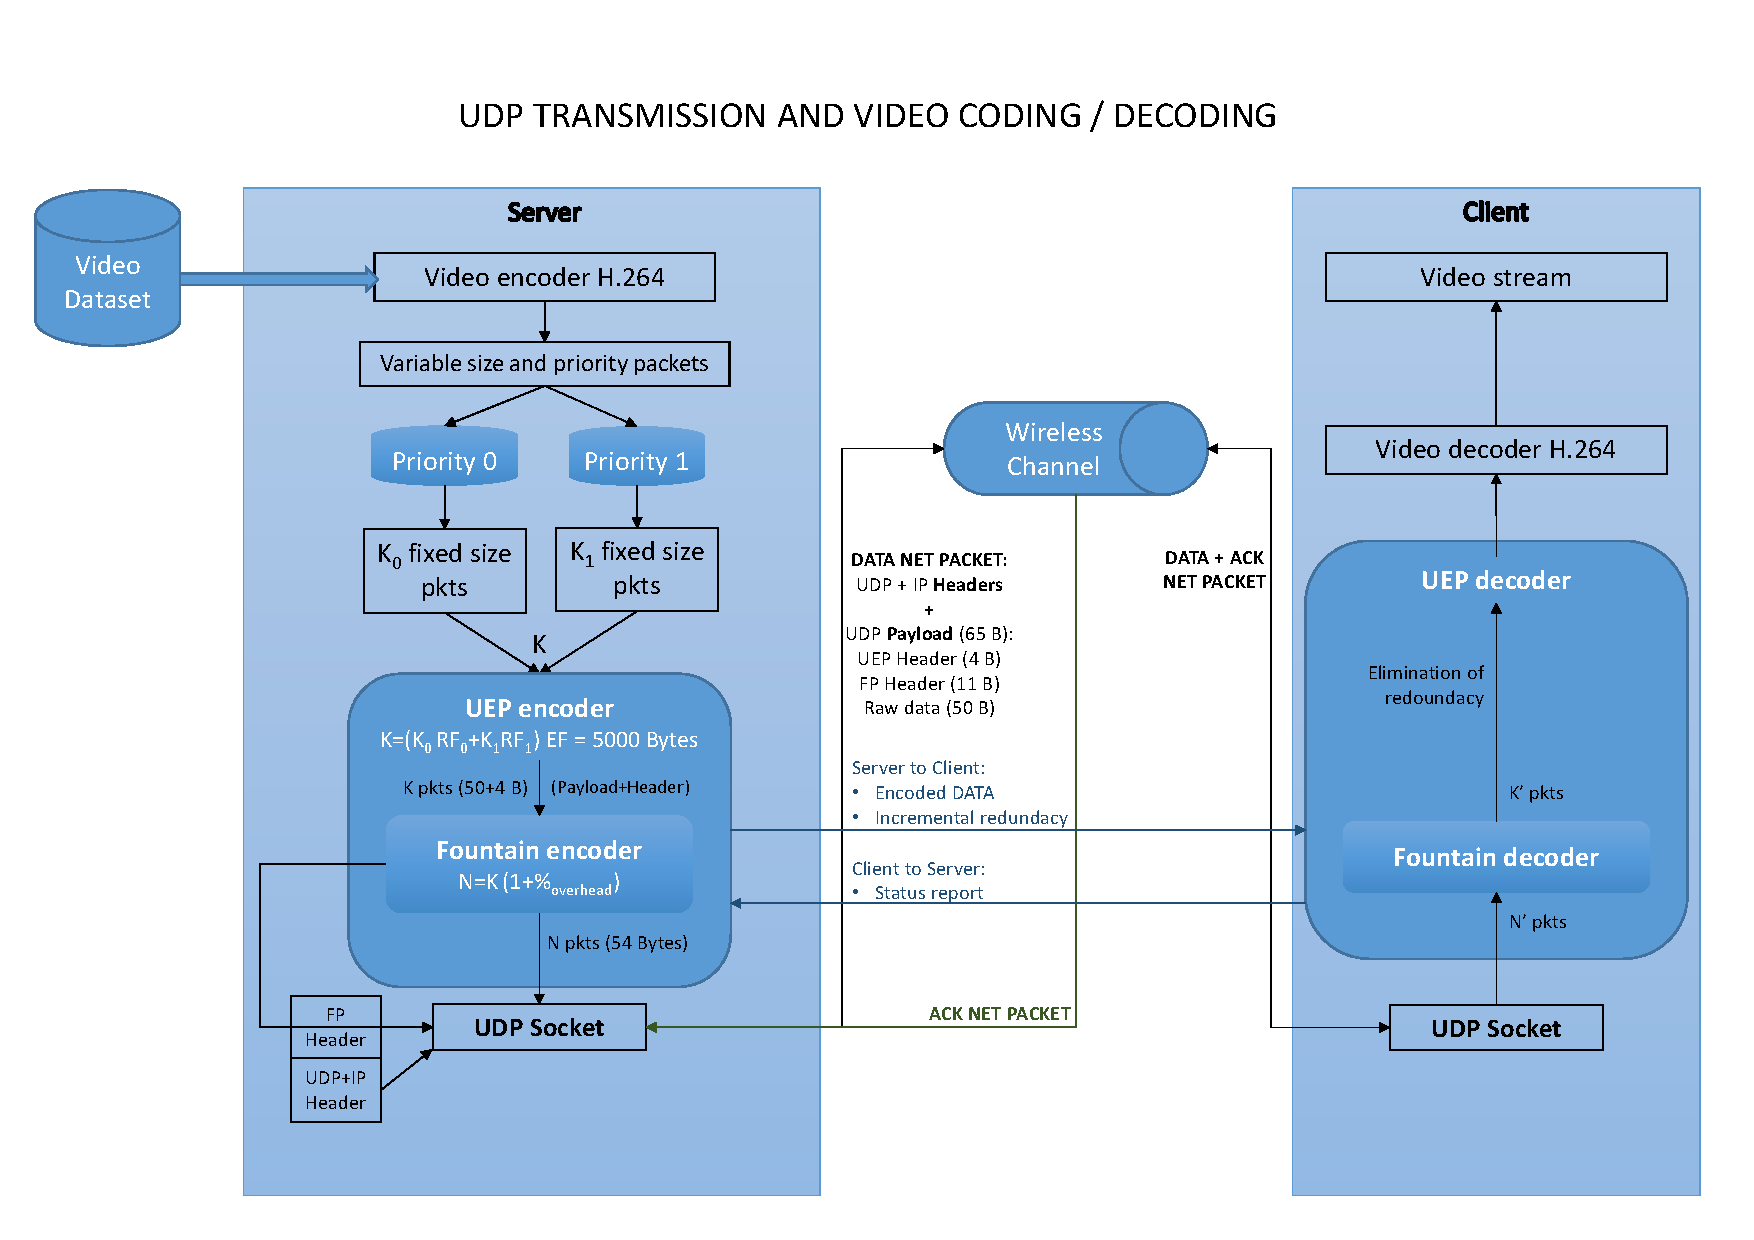
\includegraphics[clip, trim=0cm 1cm 0cm 1cm, width=1.00\textwidth]{UDP.pdf}
    \caption{Video stream encoding / decoding and transmission}
    \label{fig:UDP}
\end{figure}
% Figure TODO: elimination of redundancy -> (partially) decoded blocks [K_0, K_1]
% Then: Packet reordering ] UEP decoder -> Video decoder H264
% Remove ACK NET PACKET, Remove client to server status report
% Remove fixed packet sizes

%
%% \begin{figure}[H]
%%     \centering
%%         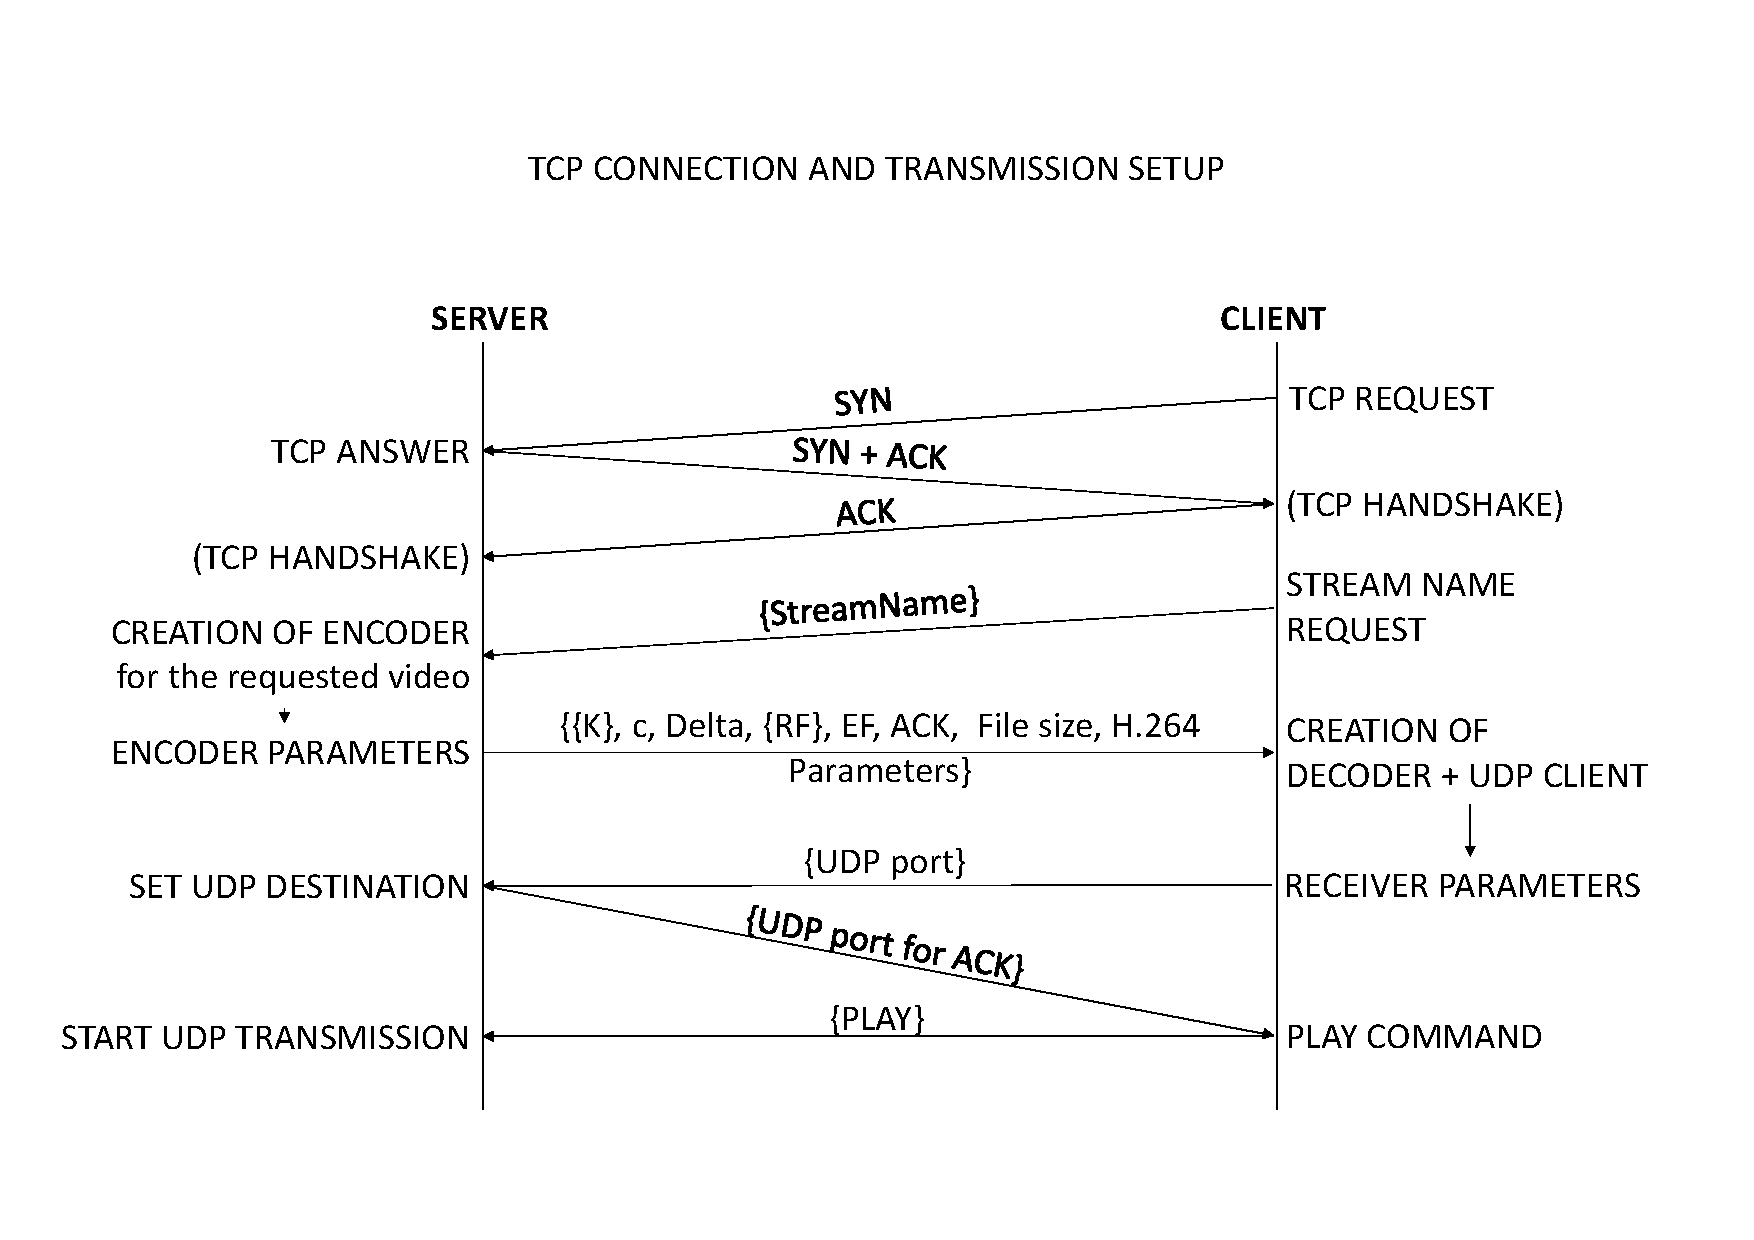
\includegraphics[clip, trim=0cm 1cm 0cm 1cm, width=1.00\textwidth]{TCP.pdf}
%%     \caption{TCP connection and tansmission setup}
%%     \label{fig:TCP}
%% \end{figure}
%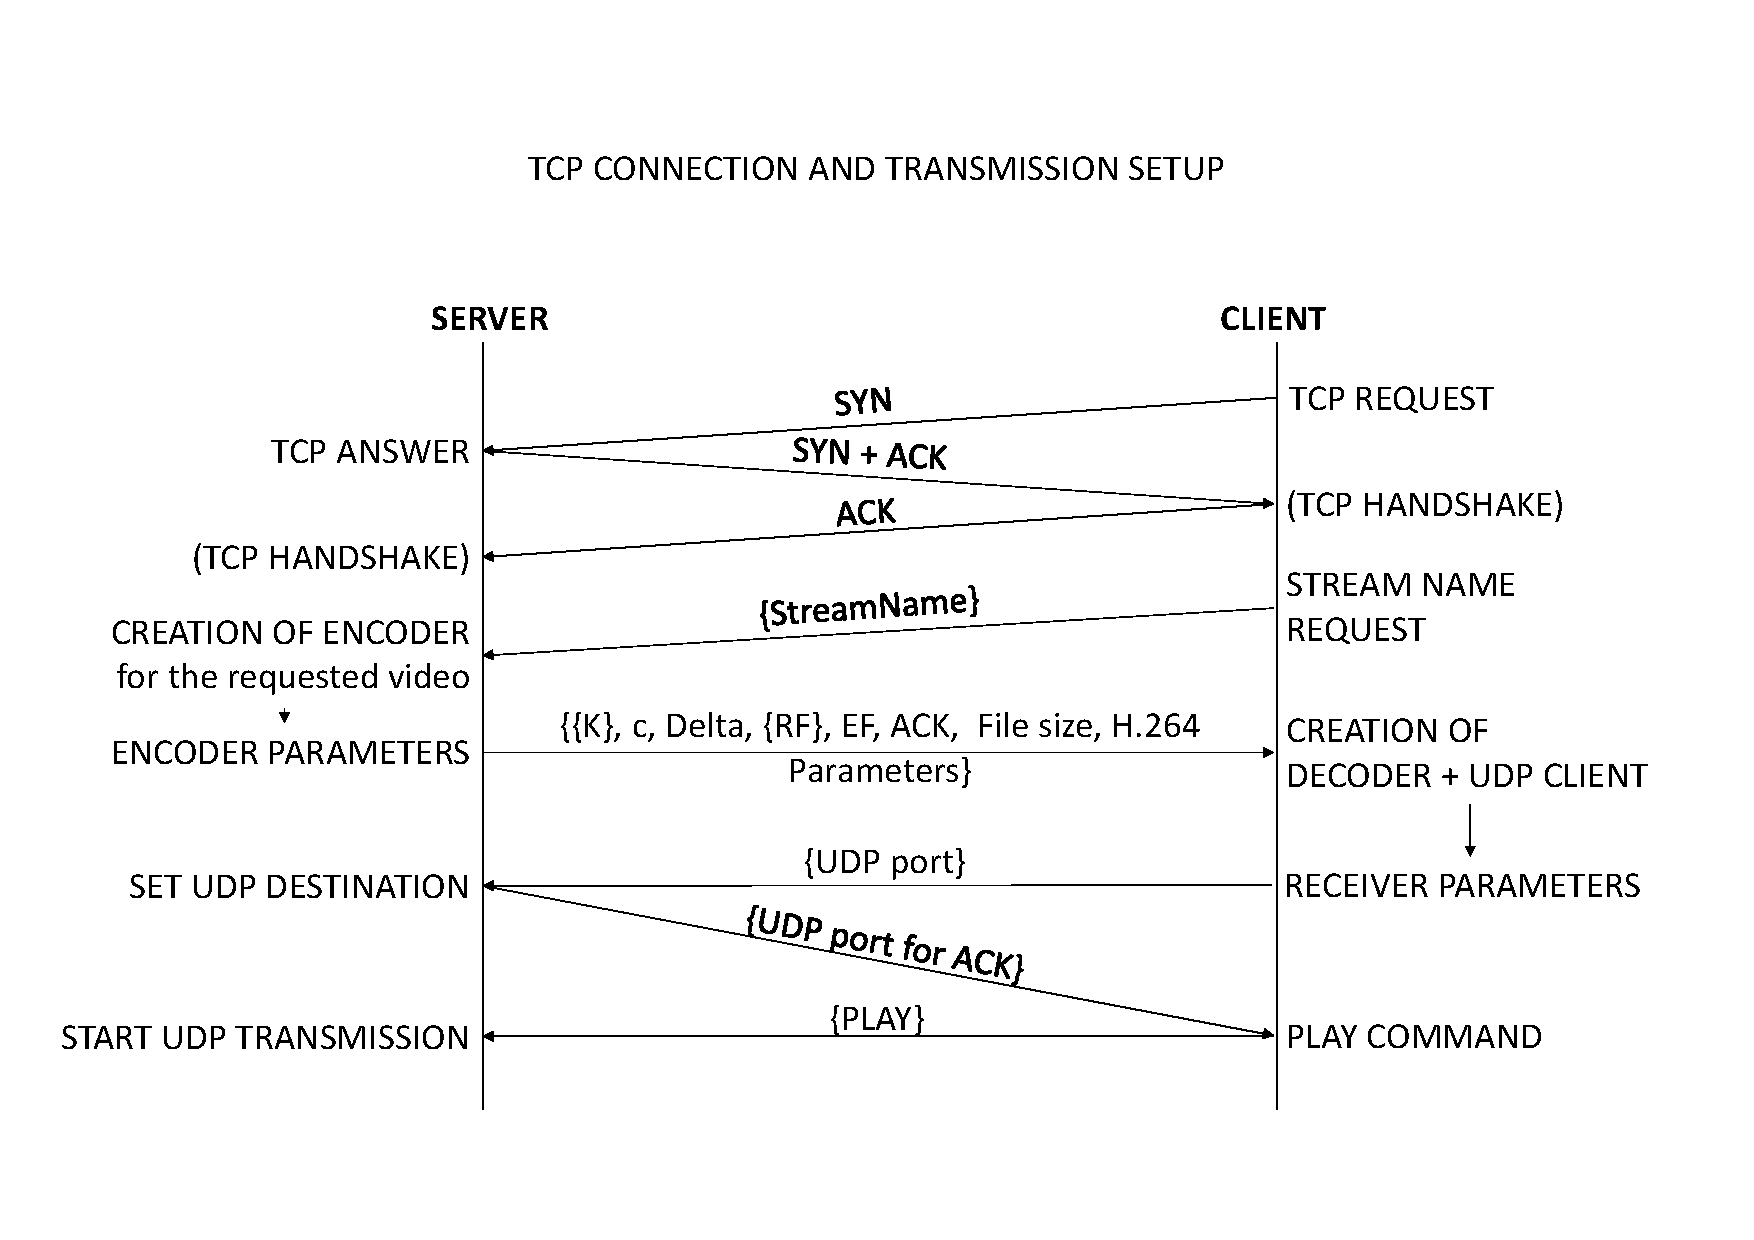
\includepdf{TCP.pdf}
\subsection{Modelli matematici}
\subsubsection{Codici a fontana}\label{FCsection}
I codici a fontana \cite{fcsurvey, rossifc} sono una classe di codici di correzione degli errori che aggiunge a un messaggio $\bm{i}\in\mathcal{A}^K$, di lunghezza $K$, una quantità di ridondanza potenzialmente infinita, aumentando la lunghezza del messaggio codificato $\bm{e}\in\mathcal{A}^N$, in modo tale che sia possibile recuperare con buona probabilità il messaggio originale da un sottoinsieme di cardinalità leggermente maggiore di $K$ del messaggio codificato.\\
%L'overhead introdotto dalla codifica è dato da $t = \frac{N-K}{K}$.\\
Fissando la lunghezza del messaggio codificato, $N$, per ogni messaggio originale di lunghezza fissata $K$, è possibile schematizzare la codifica di canale lineare attraverso la seguente equazione
\begin{equation}
\bm{e} =
\begin{pmatrix}
e_1 \\e_2 \\e_3 \\\vdots \\e_N
\end{pmatrix} = \underbrace{\begin{pmatrix}
g_{11}	&g_{12}	&\cdots	&g_{1K}\\
g_{21}	&g_{22}	&\cdots	&g_{2K}\\
g_{31}	&g_{32}	&\cdots	&g_{3K}\\
\vdots &\ddots & \ddots &\vdots\\
g_{N1}	&g_{N2}	&\cdots	&g_{NK}
\end{pmatrix}}_{=G} \begin{pmatrix}
i_1 \\i_2 \\\vdots \\i_K
\end{pmatrix} = G \cdot \bm{i}
\end{equation}
dove $G$ è la matrice di codifica, $g_{jk}\in\{0,1\}$, $i_j, e_j\in\mathcal{A}$.\\
La $j-$esima riga della matrice $G$ (detta anche $j$-esimo vettore di codifica) è generata casualmente e il suo grado (la distanza di Hamming dalla riga nulla) segue una distribuzione di probabilità nota: la Robust Soliton Distribution.\\
La codifica del $j-$esimo pacchetto avviene attraverso l'operazione di \emph{XOR} tra i pacchetti di input selezionati dagli elementi della $j-$esima riga di $G$.\\
Se $G$ è invertibile, è possibile recuperare il vettore $\bm{i}$ da $\bm{e}$ attraverso la risoluzione di un sistema lineare.\\
\begin{figure}[htb]
    \centering
        \makebox[\textwidth][c]{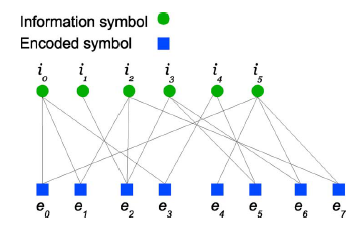
\includegraphics[width=6cm]{fc.png}}
    \caption{Schema: \textit{message passing}}
    \label{fig:FC}
\end{figure}
I codici a fontana non prevedono la risoluzione di un sistema lineare per la decodifica, bensì un algoritmo sub-ottimale ma molto più veloce detto \emph{message passing}. L'algoritmo può essere così descritto (con riferimento alla figura~\ref{fig:FC}):
\begin{itemize}
        \item SE esiste un simbolo codificato $e_n$ con un solo arco entrante (es. $e_4$)\begin{itemize}
                \item	Decodifica il simbolo di informazione corrispondente $i_k=e_n$ ($i_5$ in questo caso) e rimuovi l'arco uscente da $e_n$
                \item	Sostituisci tutti i simboli codificati $e_{n'}$ aventi un arco entrante da $i_k$ con $e_{n'}^{\text{new}} = e_{n'} \textit{ XOR } i_k$
                \item   Rimuovi gli archi uscenti da $i_k$
                \item   SE ci sono altri simboli di informazione da decodificare \begin{itemize}
                        \item Torna all'inizio
                \end{itemize}
                \item ALTRIMENTI\begin{itemize}
                        \item Decodifica riuscita
                \end{itemize}
        \end{itemize}

        \item ALTRIMENTI Decodifica fallita
\end{itemize}

Da tale descrizione si evince come sia possibile non riuscire a decodificare un blocco, anche se il canale è completamente affidabile. Da questa osservazione nasce l'interesse verso le prestazioni dell'algoritmo in condizioni di trasmissione senza errori.

\subsubsection{Protezione non uniforme dagli errori}\label{UEPsection}
La protezione non uniforme di un blocco di simboli secondo l'algoritmo esposto in \cite{uep} prevede la divisione dei simboli che lo compongono in $p$ parti di diversa importanza.
Ogni parte viene ripetuta un numero $RF_i$ di volte, con $i\in\{1,\dots,p\}$, in base alla sua importanza.
Il risultato della concatenazione delle parti ripetute viene a sua volta ripetuto un numero $EF$ di volte.
%
Il blocco di simboli che si ottiene in seguito alle ripetizioni (detto ``blocco virtuale'') è utilizzato nel processo di generazione dei vettori di codifica al posto del blocco originale.
%
I simboli di input selezionati dai vettori di codifica sono poi mappati nei simboli appartenenti al blocco originale, aumentando in tal modo la probabilità che un simbolo di output contenga uno dei simboli di input ripetuti più volte.
%
Di seguito (figura~\ref{fig:UEP}) uno schema rappresentativo con $p=2$, $RF_1 = 2$,$RF_2=1$, $EF=2$.
\begin{figure}[htb]
    \centering
        \makebox[\textwidth][c]{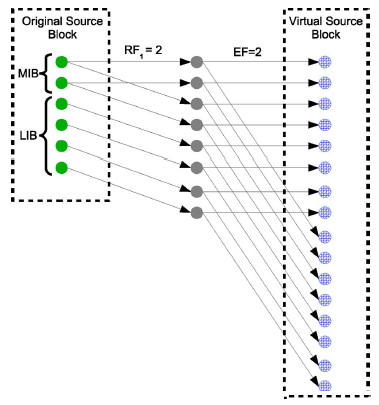
\includegraphics[width=8cm]{uep.png}}
    \caption{Schema della protezione non uniforme}
    \label{fig:UEP}
\end{figure}

%% \subsubsection{H.264}
%% Più nel dettaglio, il flusso video codificato è organizzato in unità NAL (Network Abstraction Layer) che possono essere di 2 tipi: VCL NAL Packets (Video Coding Layer) e non-VCL NAL packets. I pacchetti non-VCL possono contenere il set di parametri da usare per decodificare (informazioni necessarie per la decodifica, quindi ad alta priorità), oppure delle informazioni supplementari per migliorare la decodifica (SEI, Supplemental Enhancement Information). Il bitstream NAL è composto da una serie di sequenze video più corte (GOP, Group Of Pictures) decodificabili indipendentemente dal resto del flusso: ogni GOP comincia con tutte le informazioni necessarie alla decodifica, in modo che essa possa avvenire anche senza aver decodificato nessun segmento precedente.\\
%% Un tipo di applicazione che si presta particolarmente all'utilizzo di UEP \cite{uep} è lo streaming di un video codificato attraverso SVC, infatti tale protocollo rende possibile la decodifica di un flusso video da flussi parziali, chiamati \textit{layer}, con risoluzione spaziale o temporale minore, o con fedeltà ridotta. I layer sono ordinati dal più importante (layer 0, a bassa qualità) al meno importante (layer \textit{n}, che permette di raggiungere alta qualità).\\
%% La presenza di informazioni più rilevanti di altre (come i parametri per la decodifica e i layer inferiori, in particolare i frame intra-coded) giustifica l'uso di UEP: i flussi con priorità minore aggiungono qualità al video decodificato, ma non sono indispensabili per la decodifica, quindi possono essere protetti con meno ridondanza.

\subsubsection{Canale}
\label{sec:markov}
Il canale simulato nei test è un ``packet deletion channel'' di due
tipi: con cancellazioni iid e con cancellazioni modellate da una
catena di Markov a due stati.
%
\begin{figure}[htb]
    \centering
        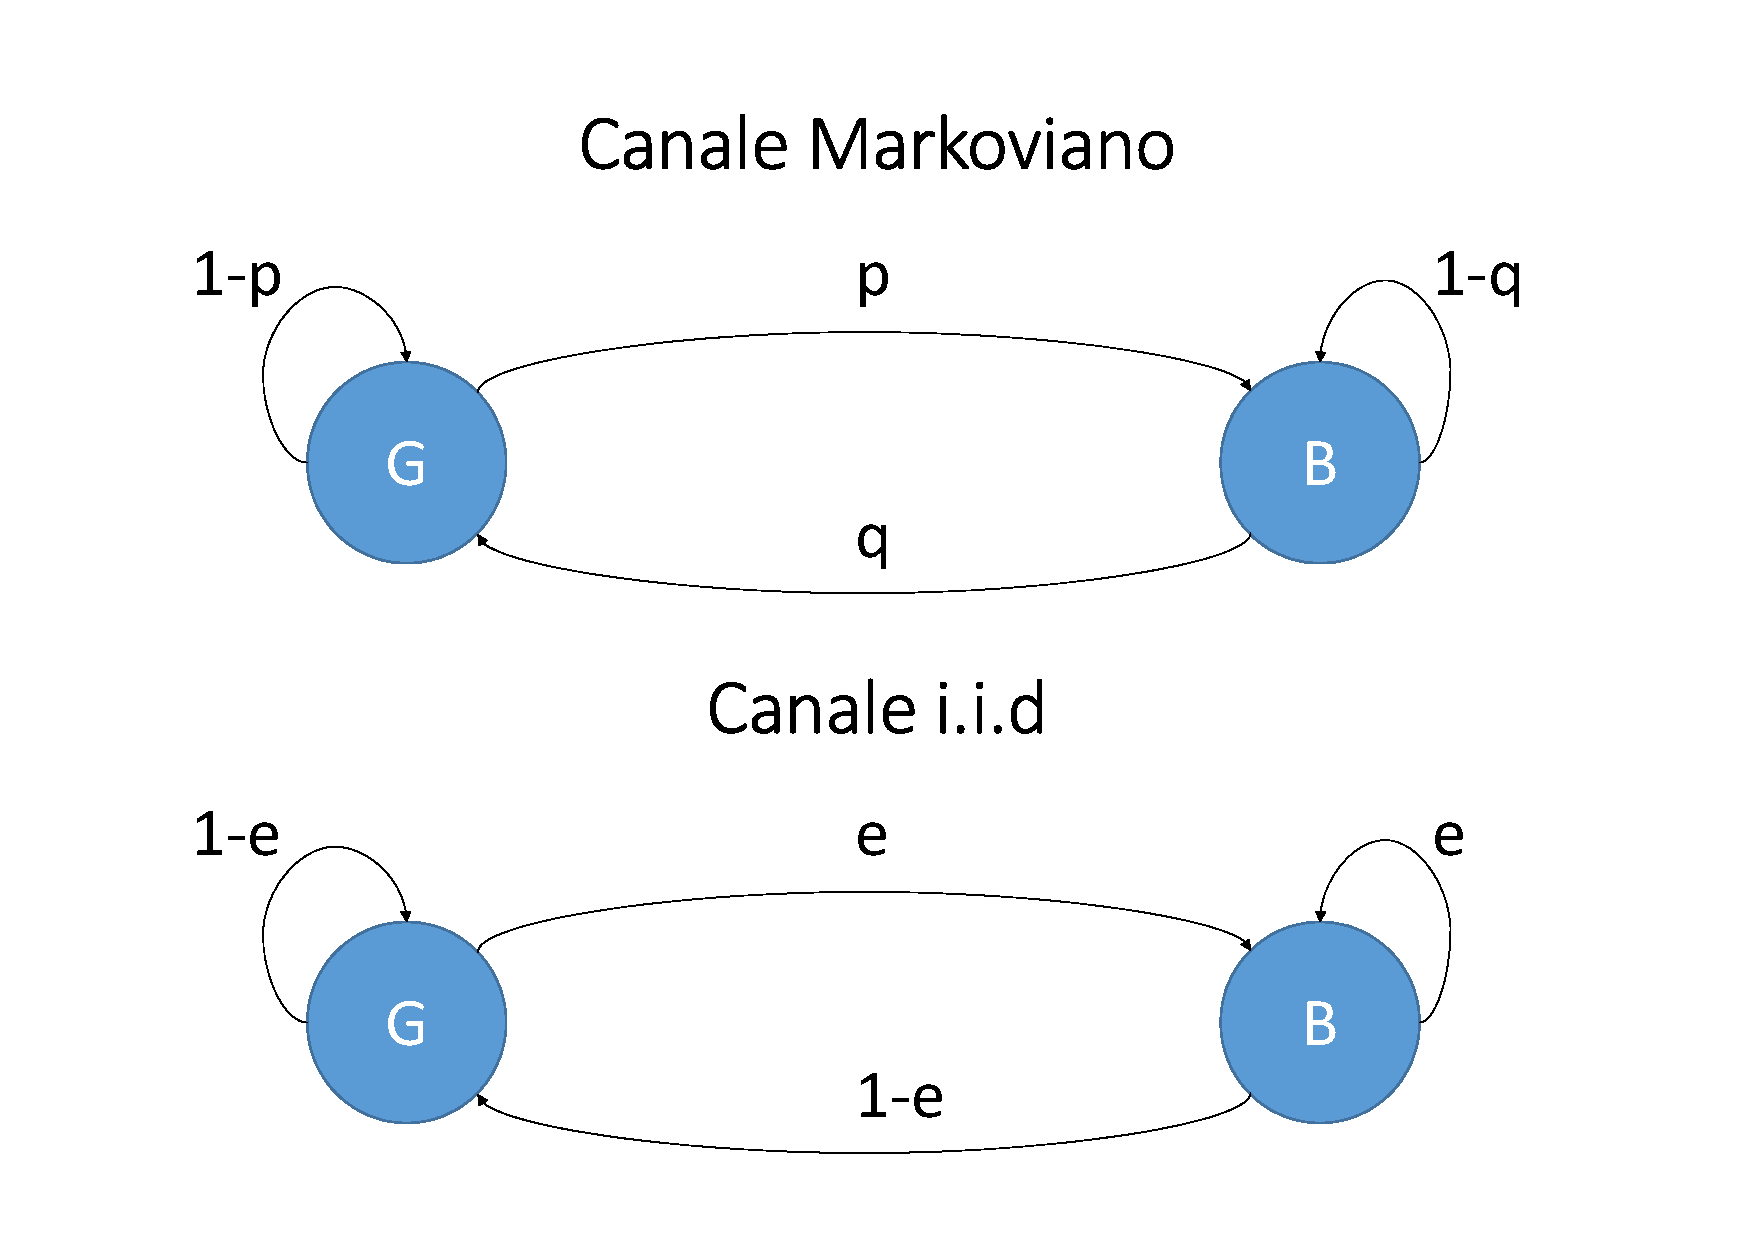
\includegraphics[clip, trim=0cm 1cm 0cm 1cm, width=0.5\textwidth]{Channel.pdf}
    \caption{Rappresentazione dei due tipi di canale utilizzati.}
    \label{fig:Channel}
\end{figure}

In quest'ultimo tipo di canale, lo stato può essere ``buono'' (G), a
cui corrisponde la ricezione corretta del pacchetto, o ``cattivo''
(B), in cui il pacchetto viene scartato.
%
Anzichè specificare direttamente le probabilità di transizione $p =
P[X_n = B | X_{n-1} = G]$ e $q = P[X_n = G | X_{n-1} = B]$ tra i due
stati, nelle simulazioni sono stati fissati altri due parametri per
caratterizzare il canale.
%
Il primo è la probabilità media di scartare un pacchetto, che
corrisposnde alla probabilità stazionaria di essere nello stato B:
\begin{equation}
  \pi_B = \frac{p}{p+q} .
\end{equation}
%
Il secondo parametro utilizzato è la lunghezza media di un burst di
cancellazioni, cioè il numero medio di transizioni necessarie ad
arrivare in G partendo da B:
\begin{equation}
  \EnB = \frac{1}{q} .
\end{equation}
%
Le probabilità di transizione possono essere poi ricavate da questi due
parametri:
\begin{equation}
  \begin{cases}
    q &= \frac{1}{\EnB} \\
    p &= q \frac{\pi_B}{1 - \pi_B}
  \end{cases}
  \label{eq:mcparams}
\end{equation}

%% Il numero medio di iterazioni necessarie a sbagliare N pacchetti è
%% \begin{equation}
%% \label{avg_errors}
%% E[\theta_{0N}] = \frac{\pi_G}{p} + \frac{N-1}{\pi_B}
%% \end{equation}

Il canale senza memoria è semplicemente un caso particolare del canale
a due stati, caratterizzato dalle seguenti probabilità di
transizione:
\begin{equation}
  \begin{cases}
    p &= e \\
    q &= 1-e
  \end{cases}
\end{equation}
dove $e$ è la probabilità iid di cancellare un pacchetto.

\subsection{Complicazioni trovate} % Max 5 lines
\label{sec:complications}
Purtroppo l'esecuzione dell'intera implementazione dello schema di
figura~\ref{fig:UDP} richiede un tempo tale da rendere difficoltosa la
costruzione di grafici che siano precisi per PER basse.
%
I risultati della sezione~\ref{sec:results} sono, quindi, stati
ottenuti applicando direttamente il message passing, senza trasmettere
realmente dei pacchetti.

\section{Risultati} % Min 7 pages
\label{sec:results}
L'algoritmo per la protezione non uniforme esposto nel
paragrafo~\ref{UEPsection} è stato testato nei due casi di canale
senza memoria e con memoria, per determinare la packet error
rate ottenibile in queste due condizioni.

Sono stati inoltre misurati i tempi necessari alla codifica e
decodifica dei pacchetti in funzione dell'overhead desiderato.

\subsection{Packet error rate su un canale senza memoria}
\label{sec:iid}
In questo caso è stata misurata la packet error rate a livello di
applicazione ottenuta variando l'overhead e considerando diversi
valori per la packet error rate del canale.
%
Facendo riferimento alla figura~\ref{fig:UDP}, la PER di livello
applicazione è la frazione di pacchetti forniti all'UEP encoder che
raggiungono l'uscita dell'UEP decoder, che corrisponde alla frazione
di pacchetti decodificati dal message passing.
%
L'overhead è definito, in modo analogo a \cite{uep}, come $t =
\frac{N-K}{K}$, dove $N$ è il numero di pacchetti codificati prodotti
per ogni blocco e $K$ è la dimensione del blocco.
%
Il canale iid è simulato scartando con probabilità $e$ ognuno degli
$N$ pacchetti codificati.

I valori per i parametri sono stati scelti come in \cite{uepother},
una versione precedente di \cite{uep}, perché permettono di
evidenziare meglio il diverso comportamento della PER relativa ai
pacchetti importanti rispetto al resto del blocco.

Sono stati usati blocchi contenenti $K_0 = 100$ pacchetti importanti e
$K_1 = 1900$ pacchetti non importanti, il blocco virtuale è stato
costruito ripetendo $RF_0 = 5$ volte il primo sotto-blocco, $RF_1 = 1$
volte il secondo ed espandendo la sequenza di pacchetti così ottenuta
di un fattore $EF = 2$. La lunghezza del blocco virtuale è quindi pari
a $EF \cdot \left( RF_0 \cdot K_0 + RF_1 \cdot K_1 \right) = 4800$
pacchetti.
%
L'overhead è stato fatto variare nell'intervallo $[0, 0.8]$, a cui
corrisponde un numero di pacchetti inviati $N \in [2000, 3600]$ per
ogni blocco di $K=K_0+K_1$ pacchetti.
%
La probabilità di errore del canale è stata impostata ai valori $e \in
\left\{10^{-2}, 10^{-1}, 3 \cdot 10^{-1} \right\}$, oltre al caso
senza errori con $e=0$.

Nelle figure~\ref{fig:zero_oh} e~\ref{fig:iid_oh} sono mostrati i
risultati della simulazione di 10000 blocchi.
%
\begin{figure}[H]
  \centering
  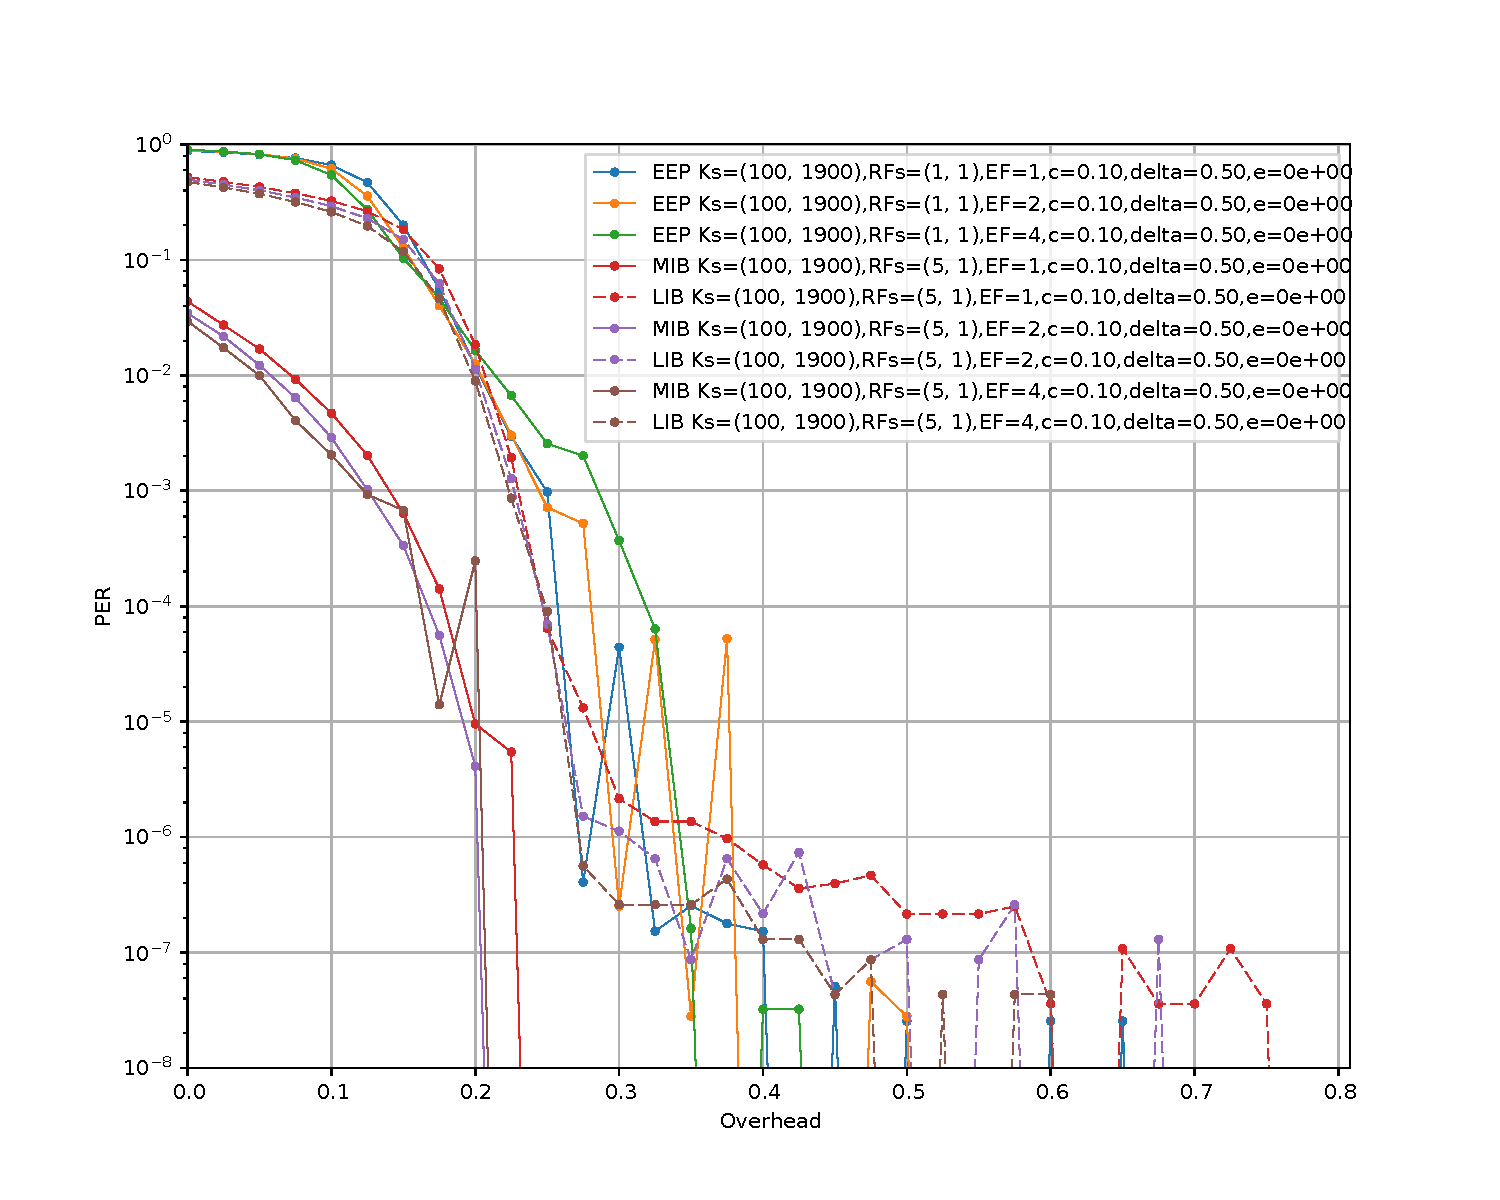
\includegraphics[width=0.8\textwidth]{plot_ber_zero_oh}
  \caption{Packet error rate al variare dell'overhead su un canale
    senza errori.}
  \label{fig:zero_oh}
\end{figure}
% Plot notes:
% better EEP EF=1 for 0.2 - 0.4 -> [8:17] or more
% Remove EEP EF>1 because worse PER after oh=0.18
% UEP EF = 4: better points in [4:17]
% UEP EF = 2: better points in [11:17]
%
\begin{figure}[H]
  \centering
  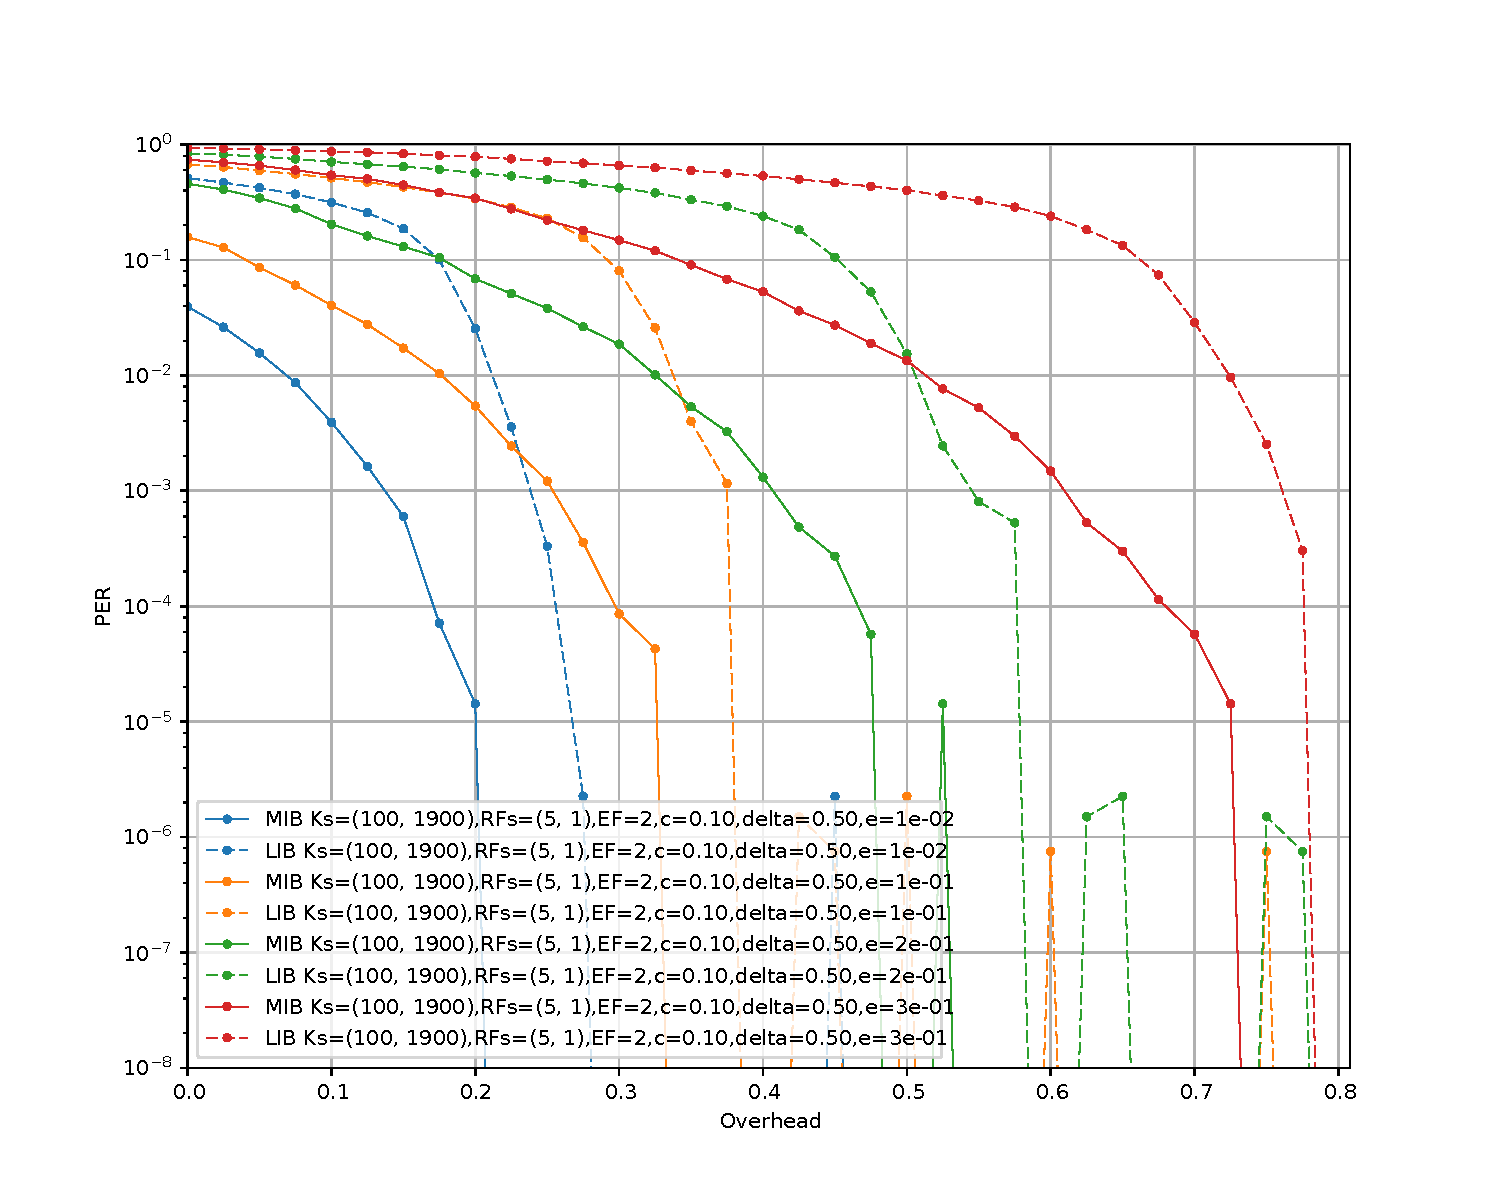
\includegraphics[width=0.8\textwidth]{plot_ber_iid}
  \caption{Packet error rate al variare dell'overhead su un canale
    iid.}
  \label{fig:iid_oh}
\end{figure}
% Plot notes:
% more points everywhere

% Markov plot notes:
% Error-free:
% EEP is good, more between 2000-4000 -> [8:12]
% UEP RF=5 more points everywhere for the LIB +
%   [4:9]
%
% BR5:
%

Nel caso senza errori (figura~\ref{fig:zero_oh}) si può vedere come la
scelta dei vettori di codifica che predilige i pacchetti importanti
fornisca un miglioramento nella PER relativa a questi ultimi, rispetto
al caso EEP.
%
D'altro canto vediamo come la PER relativa ai pacchetti meno
importanti, anche se inizialmente è migliore del caso EEP, al crescere
dell'overhead decresce più lentamente e rimane sopra a $10^{-8}$ per
tutto l'intervallo considerato.
%
Il fattore di espansione $EF$ non fornisce miglioramenti significativi
della PER del MIB, mentre permette di diminuire la PER del LIB per gli
overhead più alti. Con $EF > 2$, tuttavia, questo effetto tende a
diventare sempre più piccolo.

Dal grafico delle PER per il caso in cui il canale perde pacchetti in
modo iid (figura~\ref{fig:iid_oh}) è possible vedere che le curve
seguono un andamento simile al caso precedente, ma traslato.
Si nota come, al variare della PER del canale, l'entità della traslazione
sia di circa $1.6$ volte il valore della PER.
%
Infatti, nel caso $e = 10^{-2}$ l'algoritmo testato ha delle
prestazioni molto vicine a quelle ottenibili sul canale senza errori,
mentre nei casi con PER $e = 10^{-1}$ ed $e = 3\cdot 10^{-1}$ le curve
siano traslate, rispettivamente, circa di $0.16$ e $0.48$ rispetto al
caso senza errori.

\subsection{Packet error rate su un canale Markoviano}
Nel caso del canale Markoviano, descritto nel
paragrafo~\ref{sec:markov}, sono state eseguite simulazioni per
valutare la packet error rate considerando canali con diverse
lunghezze medie $E[\#_B]$ di una sequenza di slot cattivi consecutivi
e variando la dimensione del blocco $K$.
%
In modo analogo al paragrafo precedente, il canale è stato simulato
facendo una transizione di stato prima di ogni nuovo pacchetto e
scartando quest'ultimo in caso lo stato sia ``cattivo''. Lo stato
iniziale del canale è stato scelto, per ogni blocco di pacchetti,
secondo le probabilità stazionarie $\pi_G$ e $\pi_B$.

La frazione di pacchetti importanti presente in ogni blocco è stata
mantenuta al 5\%, come per il caso iid, e anche per gli altri
parametri sono stati usati valori simili: $RF_0 = 5$, $RF_1 = 1$,
$EF=2$, $c=0.1$, $\delta=0.5$. Il numero di pacchetti trasmessi $N$ è
stato fissato per avere un overhead del 30\%.

Dato che la PER varia con $K$ anche senza cambiare il canale, sono
state eseguite delle simulazioni al variare della dimensione del
blocco su un canale error-free. Nella figura~\ref{fig:markov_zero} si
può vedere l'andamento della PER in questo caso e confrontarla con
quella ottenuta su canali Markoviani.
%
\begin{figure}[H]
  \centering
  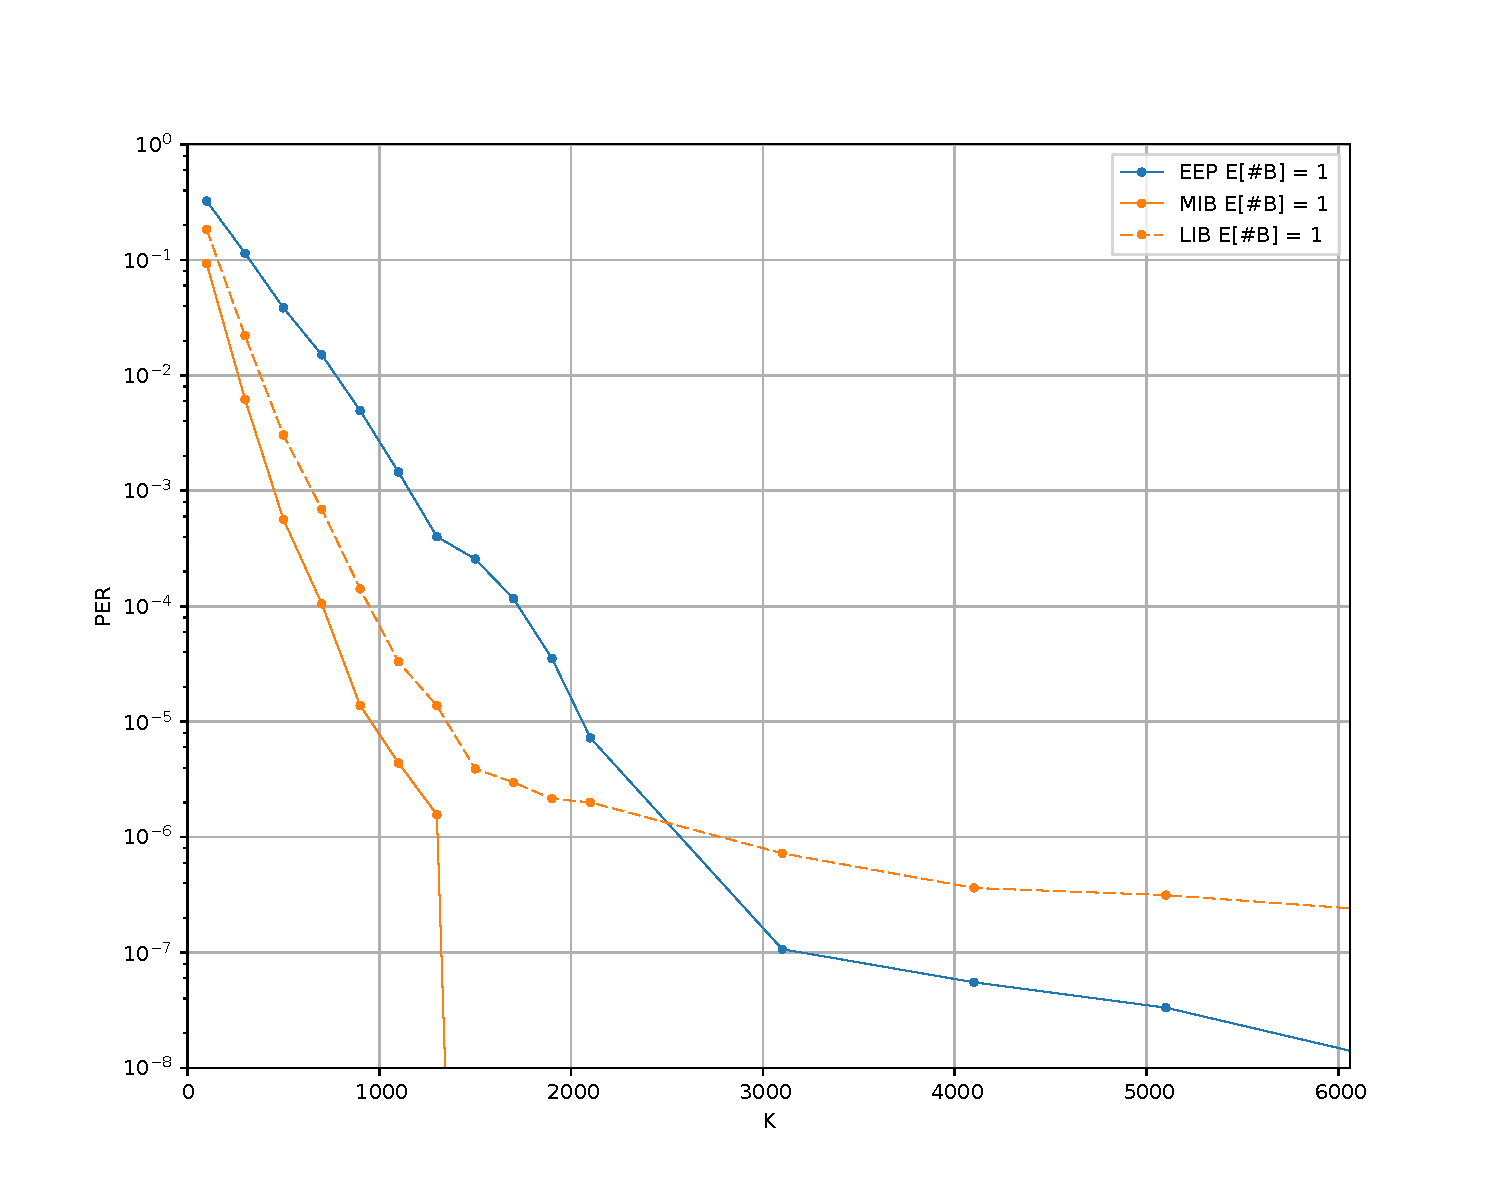
\includegraphics[width=\textwidth]{plot_markov_zero}
  \caption{Packet error rate a livello applicazione ottenuta al
    variare della dimensione del blocco sul canale error-free.}
  \label{fig:markov_zero}
\end{figure}
%
Anche nel caso del canale perfetto la probabiltà di errore è molto
alta in corrisponenza di blocchi piccoli e si può vedere come, nel
caso sia applicata la UEP, sia possibile ottenere PER basse per il MIB
molto prima che nel caso EEP.

Se, invece, consideriamo dei canali Markoviani fissando $\EnB \in
\{5,50,500\}$ e provando due diversi valori per la probabilità media
di errore $\pi_B \in \{0.01, 0.1\}$, possiamo vedere come gli errori
correlati influiscano sulla PER.
%
\begin{figure}[H]
  \centering
  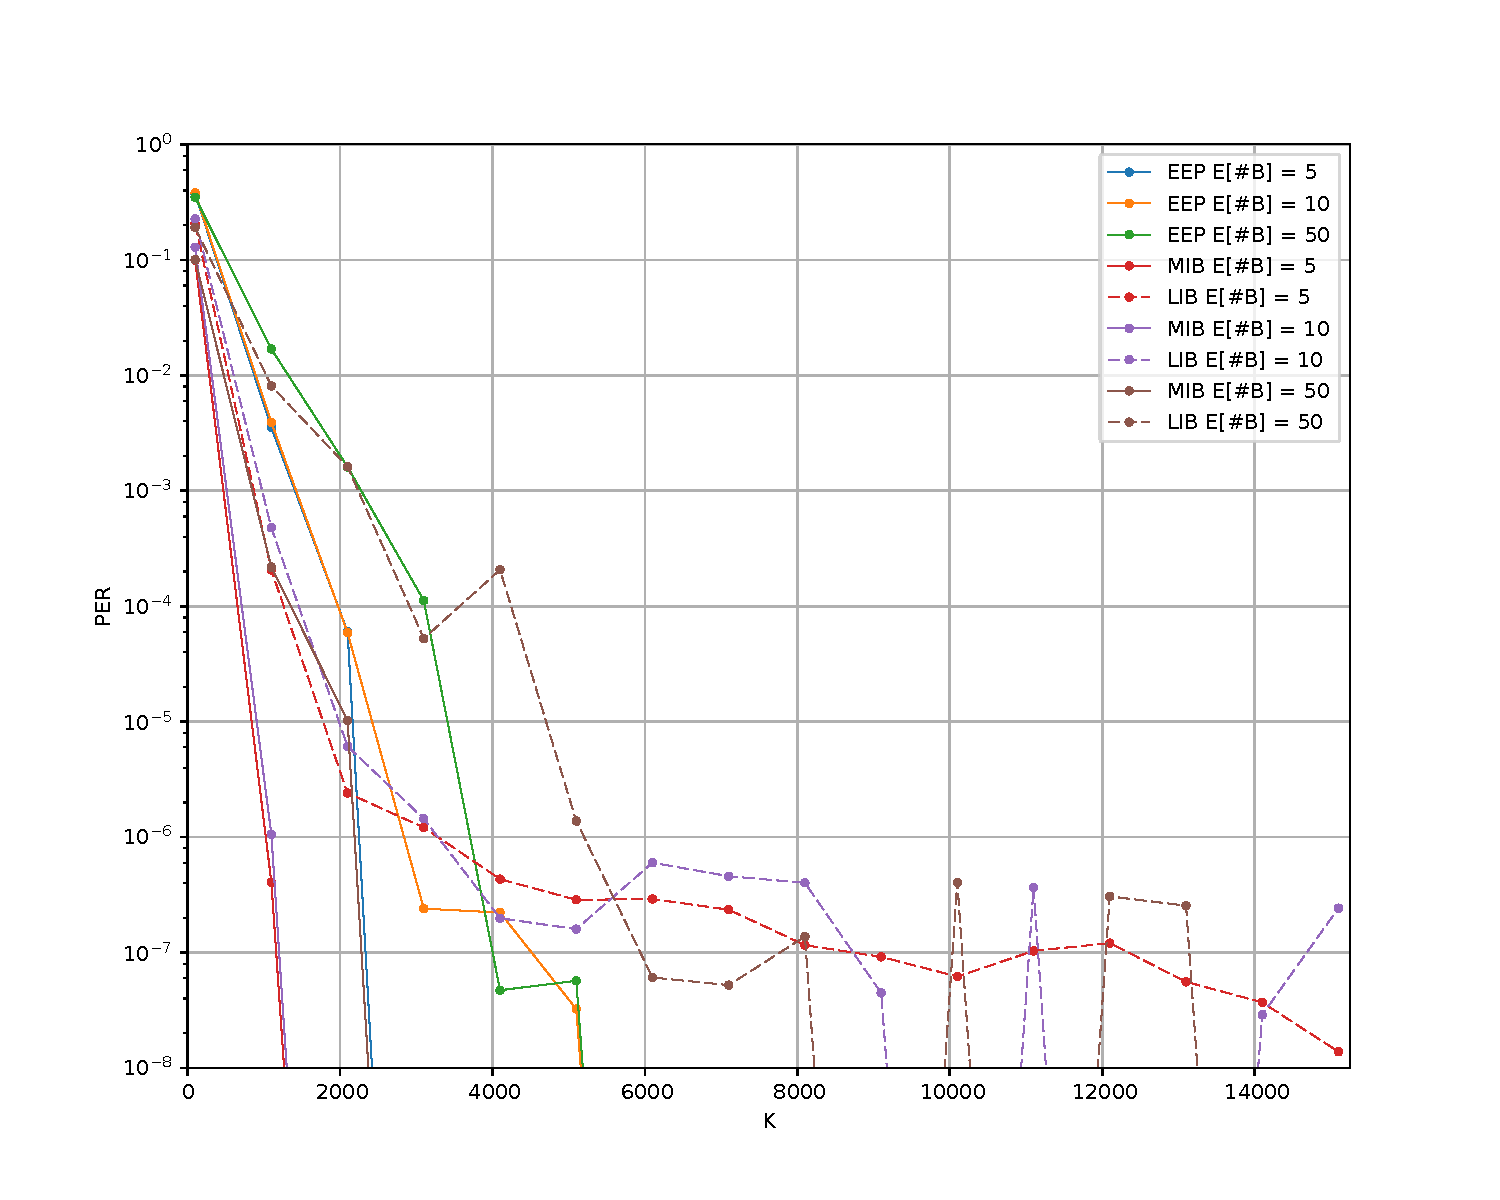
\includegraphics[width=\textwidth]{plot_markov_pi100small}
  \caption{Canale $\pi_B = 10^{-2}$, $\EnB \in \{5, 10, 50\}$}
  \label{fig:markov_pi100small}
\end{figure}
\begin{figure}[H]
  \centering
  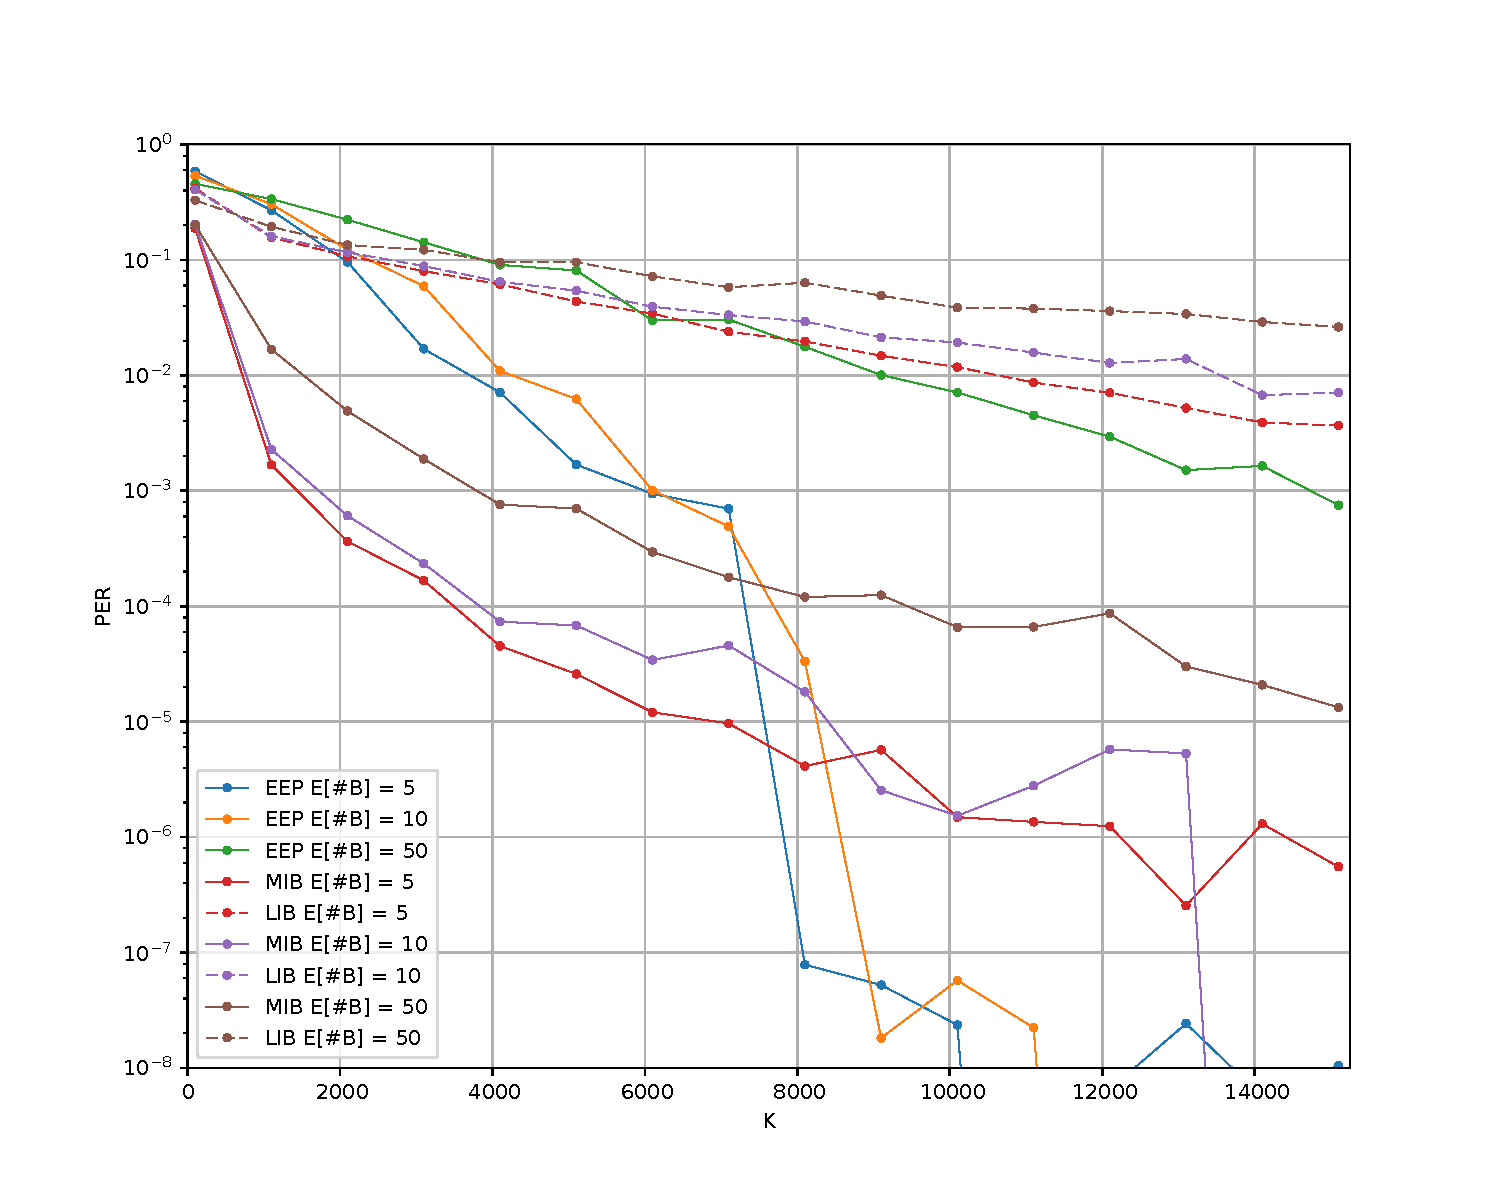
\includegraphics[width=\textwidth]{plot_markov_pi10small}
  \caption{Canale $\pi_B = 10^{-1}$, $\EnB \in \{5, 10, 50\}$}
  \label{fig:markov_pi10small}
\end{figure}
\begin{figure}[H]
  \centering
  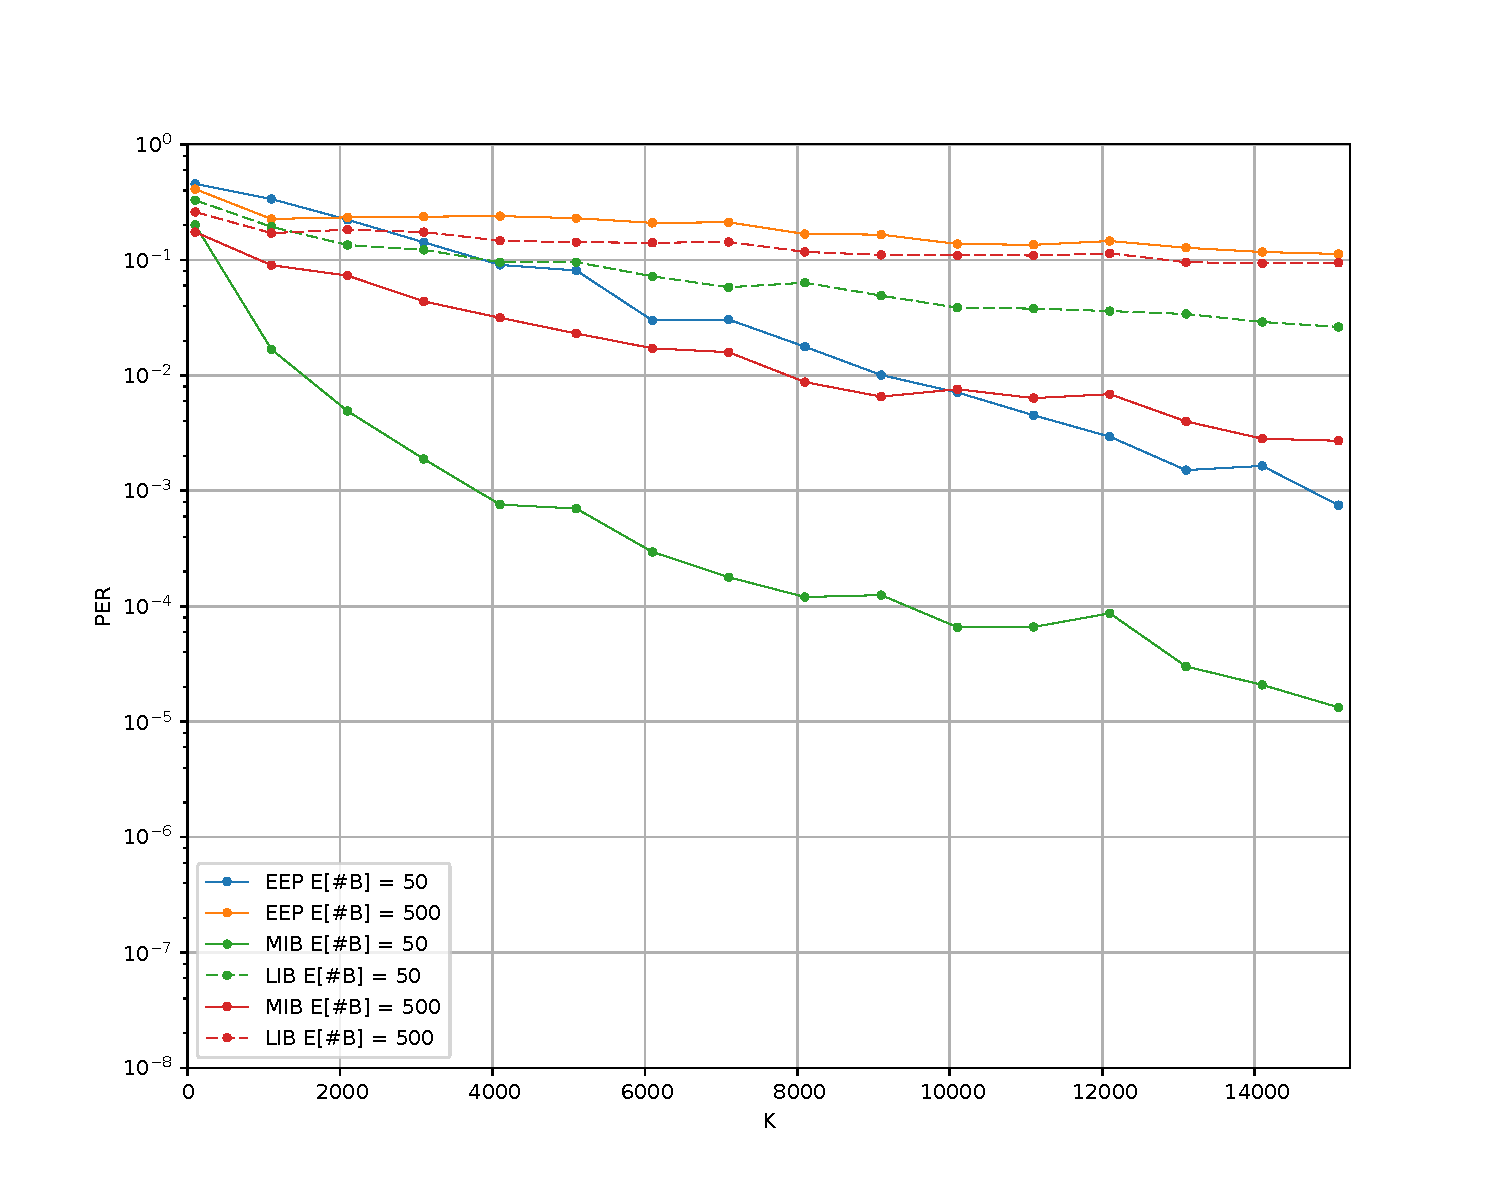
\includegraphics[width=\textwidth]{plot_markov_pi10big}
  \caption{Canale $\pi_B = 10^{-1}$, $\EnB \in \{50, 500\}$}
  \label{fig:markov_pi10big}
\end{figure}
Dai grafici sopra riportati si può notare come l'aumento della probabilità d'errore
media del canale comporti un aumento della Packet Error Rate, anche se confrontando le
figure \ref{fig:markov_zero} e \ref{fig:markov_pi100small} si nota che la differenza tra un canale
error free e un canale con probablità d'errore media $\pi_B = 10^{-1}$ è esigua.\\
Inoltre, per tutti i canali testati, fino a blocchi di dimensione $K \approx 2100$ pacchetti, 
la protezione non uniforme ha
prestazioni migliori della protezione uniforme sia per quanto riguarda la
parte più importante (MIB) che per quanto riguarda la parte meno importante (LIB).\\
Per valori di $K$ superiori, il MIB (UEP) ha una PER inferiore a quella della protezione uniforme (EEP)
mentre il LIB ha una PER superiore.\\

%
%Per canali sufficientemente buoni, in media, ma con errori più correlati,
%($\pi_B = 10^{-2}$ e $\EnB = 50$) le prestazioni in termini di PER del LIB sono
%peggiori rispetto al caso di protezione uniforme.
%
%D'altra parte, se la perdita di informazioni contenute nel LIB è meno
%rilevante rispetto alla perdita di informazioni contenute nella MIB,
%anche per canali con errori più correlati è possibile sfruttare l'algoritmo
%di protezione non uniforme al fine di mantenere la dimensione del blocco
%contenuta

%Se il canale offre una packet error rate media di $0.01$, possiamo
%notare come il peggioramento delle prestazioni rispetto ai casi
%error-free e iid (figura~\ref{fig:iid_oh}) non sia drastico per burst contenuti: la PER
%EEP scende a $10^{-8}$ in corrispondenza di $K \approx 2500,
%5000$, rispettivamente, per le tre lunghezze medie del burst; inoltre
%in tutti e tre i casi il MIB ottiene un tasso di errore più basso del
%caso EEP e peggiora altrettanto lentamente. Il LIB risente della
%correlazione tra errori nello stesso modo: le curve scendono più tardi
%a valori comparabili al caso error-free, ma la dimensione di blocco
%necessaria non è molto più alta.

%Per il caso con $\pi_B = 0.1$, invece, vediamo come la discesa della
%PER sia molto più lenta. Per $K = 2000$ possiamo confrontare il
%grafico con il caso iid e vedere come il peggioramento sia visibile ma
%non di grande entità. Rispetto al caso con $\pi_B = 0.01$, tuttavia,
%le PER del caso UEP scendono molto lentamente: il LIB non riesce a
%scendere sotto $10^{-3}$ nell'intervallo di $K$ considerato anche per
%il burst più corto, e il MIB richiede blocchi molto più grandi per
%scendere sotto $10^{-8}$. In questo caso le prestazioni della codifica
%EEP, anche se inizialmente sono peggiori del LIB, scendono più
%velocemente del MIB e permettono di ottenere una PER sotto $10^{-8}$
%con blocchi più corti di quelli richiesti per il MIB.

%Da tutto ciò possiamo vedere come, nel caso di errori correlati,
%l'effetto della protezione non uniforme sia tanto più forte quanto
%maggiore è la dimensione $K$ del blocco.
%% Il contrario, invece, accade nel caso error-free dove, al crescere
%% della dimensione del blocco, le probabilità di errore su MIB e LIB
%% tendono ad avvicinarsi \cite{uep}.

%Si vede anche come la codifica riesca a correggere bene i burst di
%errori quando la probabilità media di errore del canale non è molto
%alta, infatti la PER raggiunge velocemente valori simili al caso IID e
%offre una protezione dagli errori per il MIB migliore del caso EEP.
%
%Se la PER del canale è alta rispetto all'overhead introdotto dalla
%codifica, invece, le prestazioni sono drasticamente peggiori ed è
%necessaria una dimensione di blocco molto alta per ottenere PER basse
%sul MIB. In questo caso la codifica EEP diventa preferibile dopo una
%certa dimensione del blocco.

\subsection{Tempi di codifica e decodifica}
Per verificare quanto tempo è necessario alla codifica e alla
decodifica di un blocco di pacchetti al variare della grandezza del
blocco virtuale, è stata simulata la trasmissione di 5000 blocchi al
variare dell'overhead, utilizzando lo stesso procedimento dei
paragrafi precendenti.

Sono stati simulati sia il caso di equal error protection che quello
di unequal error protection, usando diversi valori per il fattore di
espansione $EF \in \{ 1,2,4,8,16 \}$.
%
Gli altri parametri sono gli stessi dei paragrafi precedenti: $K =
2000$, $K_0 = K \cdot 0.05$, $c=0.1$, $\delta=0.5$ e per il caso UEP
$RF_0 = 5$.

In figura~\ref{fig:encdec} sono mostrati i tempi medi di codifica e di
decodifica ottenuti eseguendo le simulazioni su un computer con CPU
Intel Xeon E5450 e con 16 GB di RAM.
%
\begin{figure}[H]
  \centering
  \begin{subfigure}{0.5\textwidth}
    \centering
    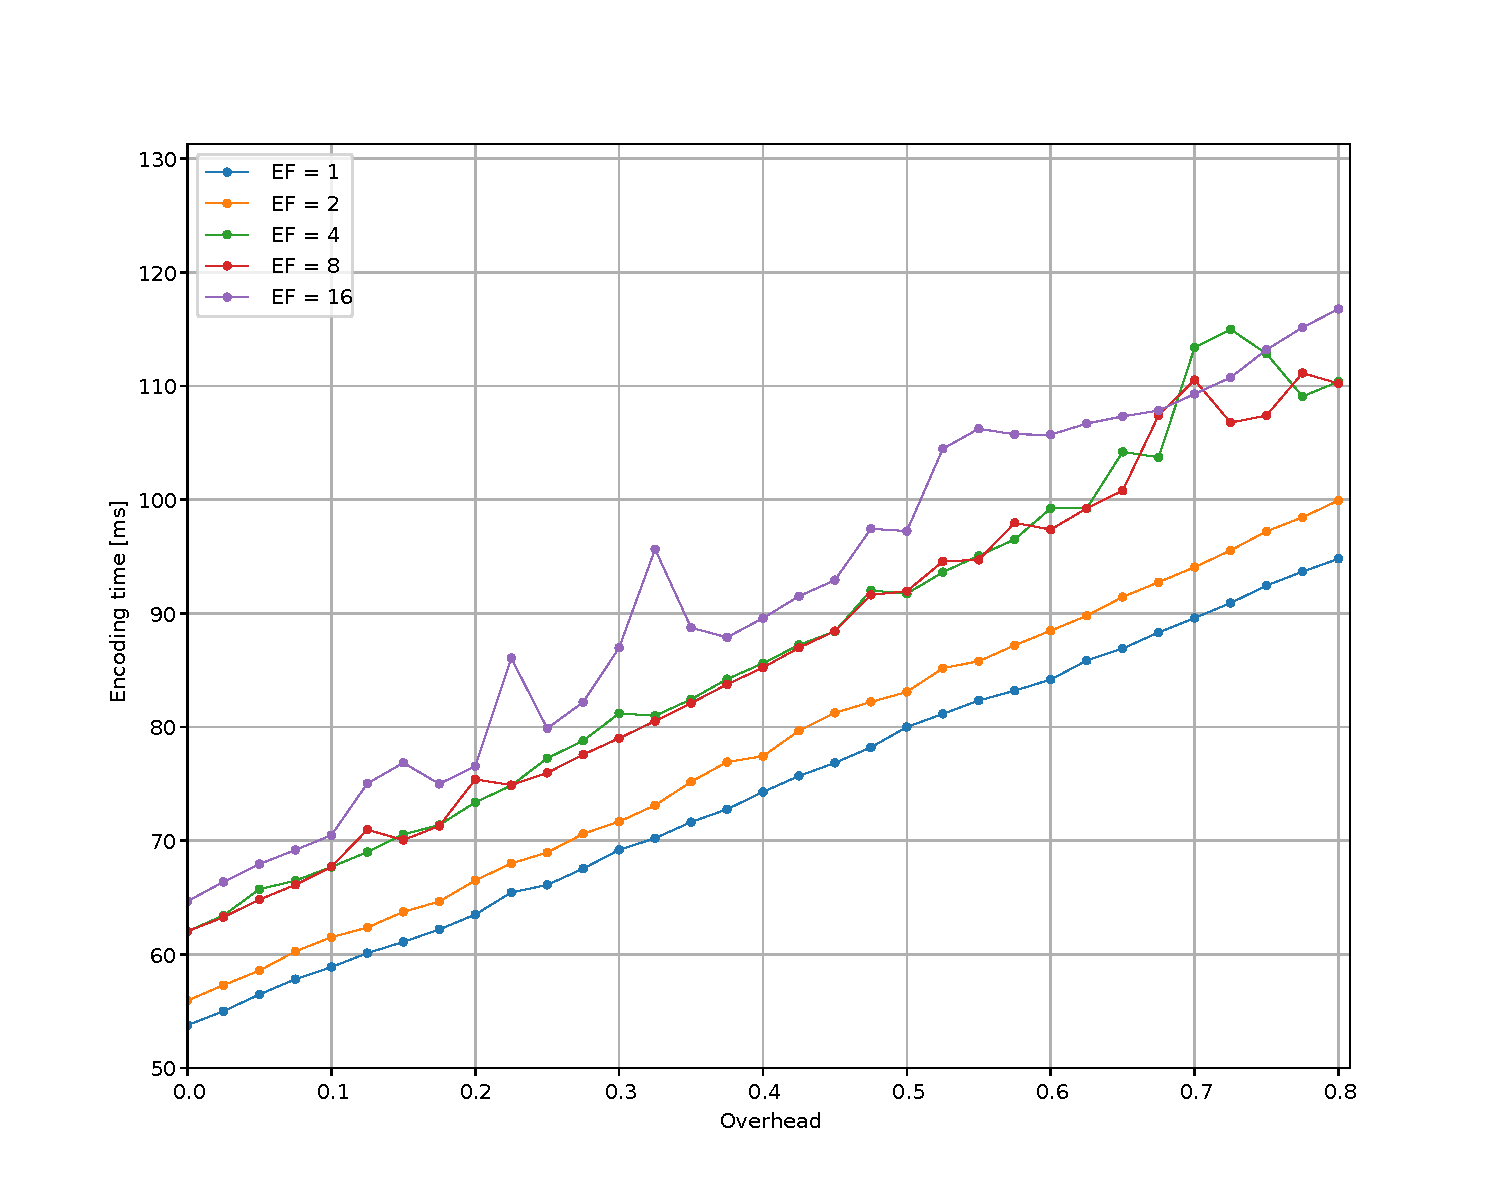
\includegraphics[width=\textwidth]{plot_enc_time_eep}
    \caption{Codifica EEP}
    \label{fig:enctime_eep}
  \end{subfigure}%
  \begin{subfigure}{0.5\textwidth}
    \centering
    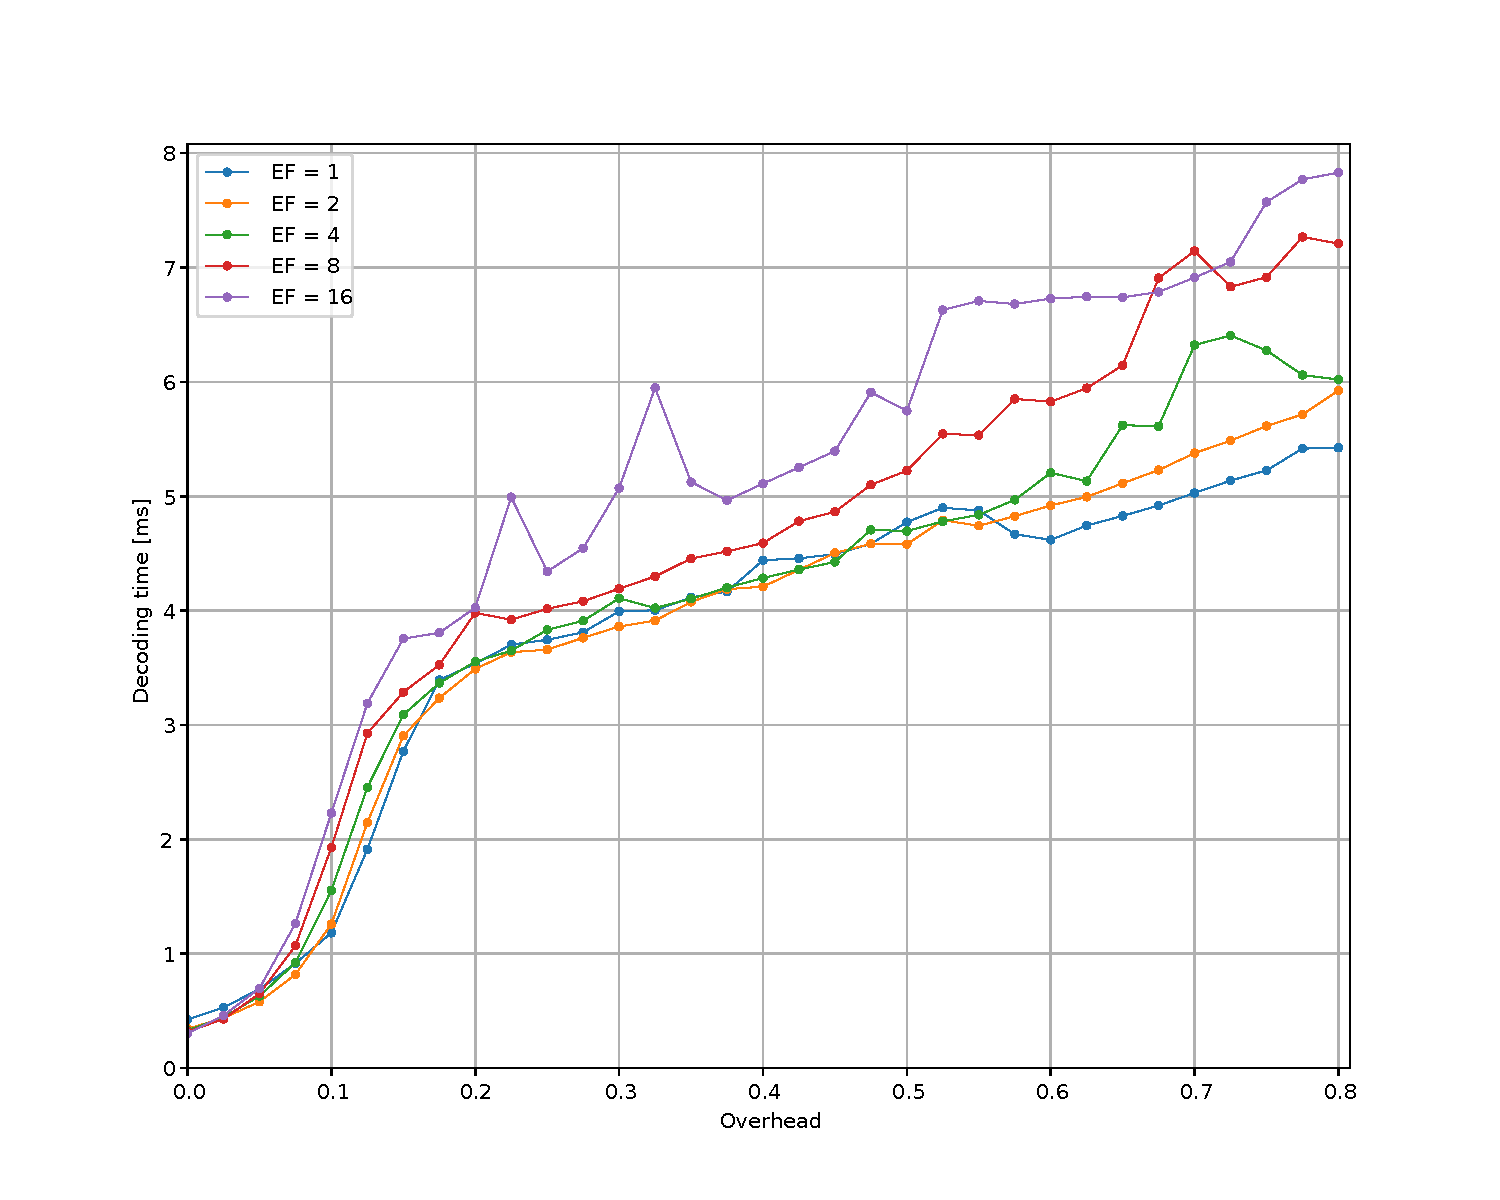
\includegraphics[width=\textwidth]{plot_dec_time_eep}
    \caption{Decodifica EEP}
    \label{fig:dectime_eep}
  \end{subfigure}
  \begin{subfigure}{0.5\textwidth}
    \centering
    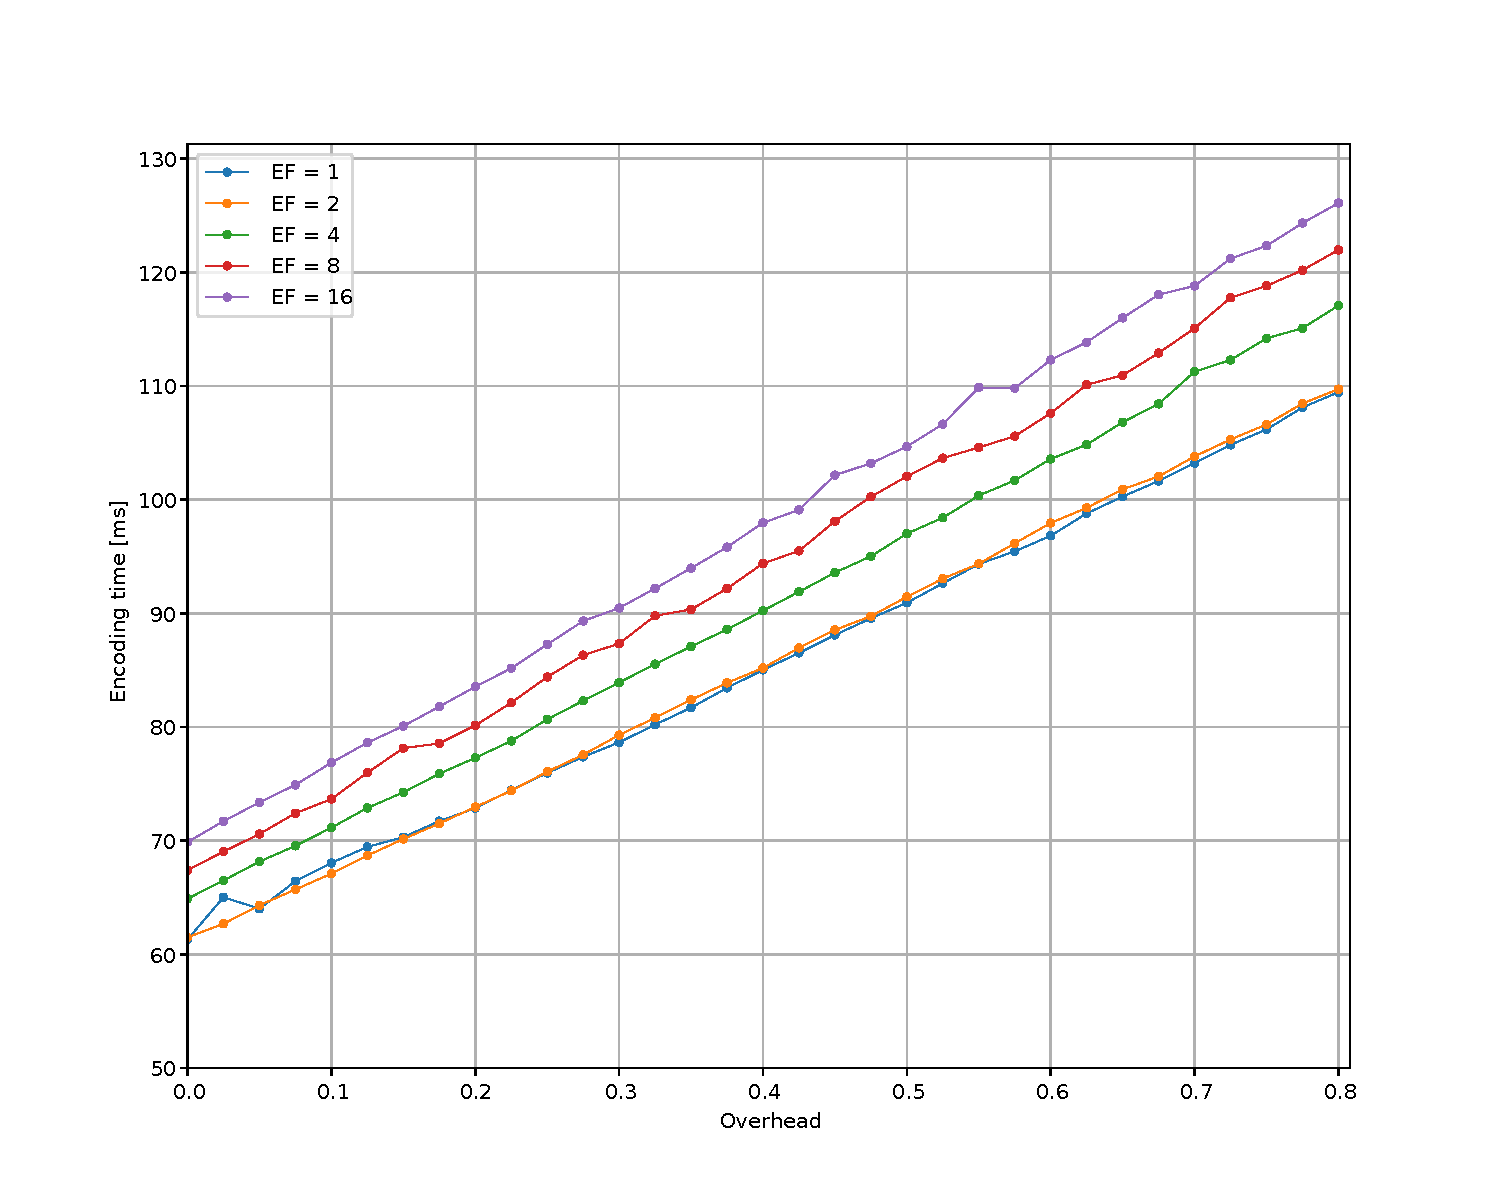
\includegraphics[width=\textwidth]{plot_enc_time_uep}
    \caption{Codifica UEP}
    \label{fig:enctime_uep}
  \end{subfigure}%
  \begin{subfigure}{0.5\textwidth}
    \centering
    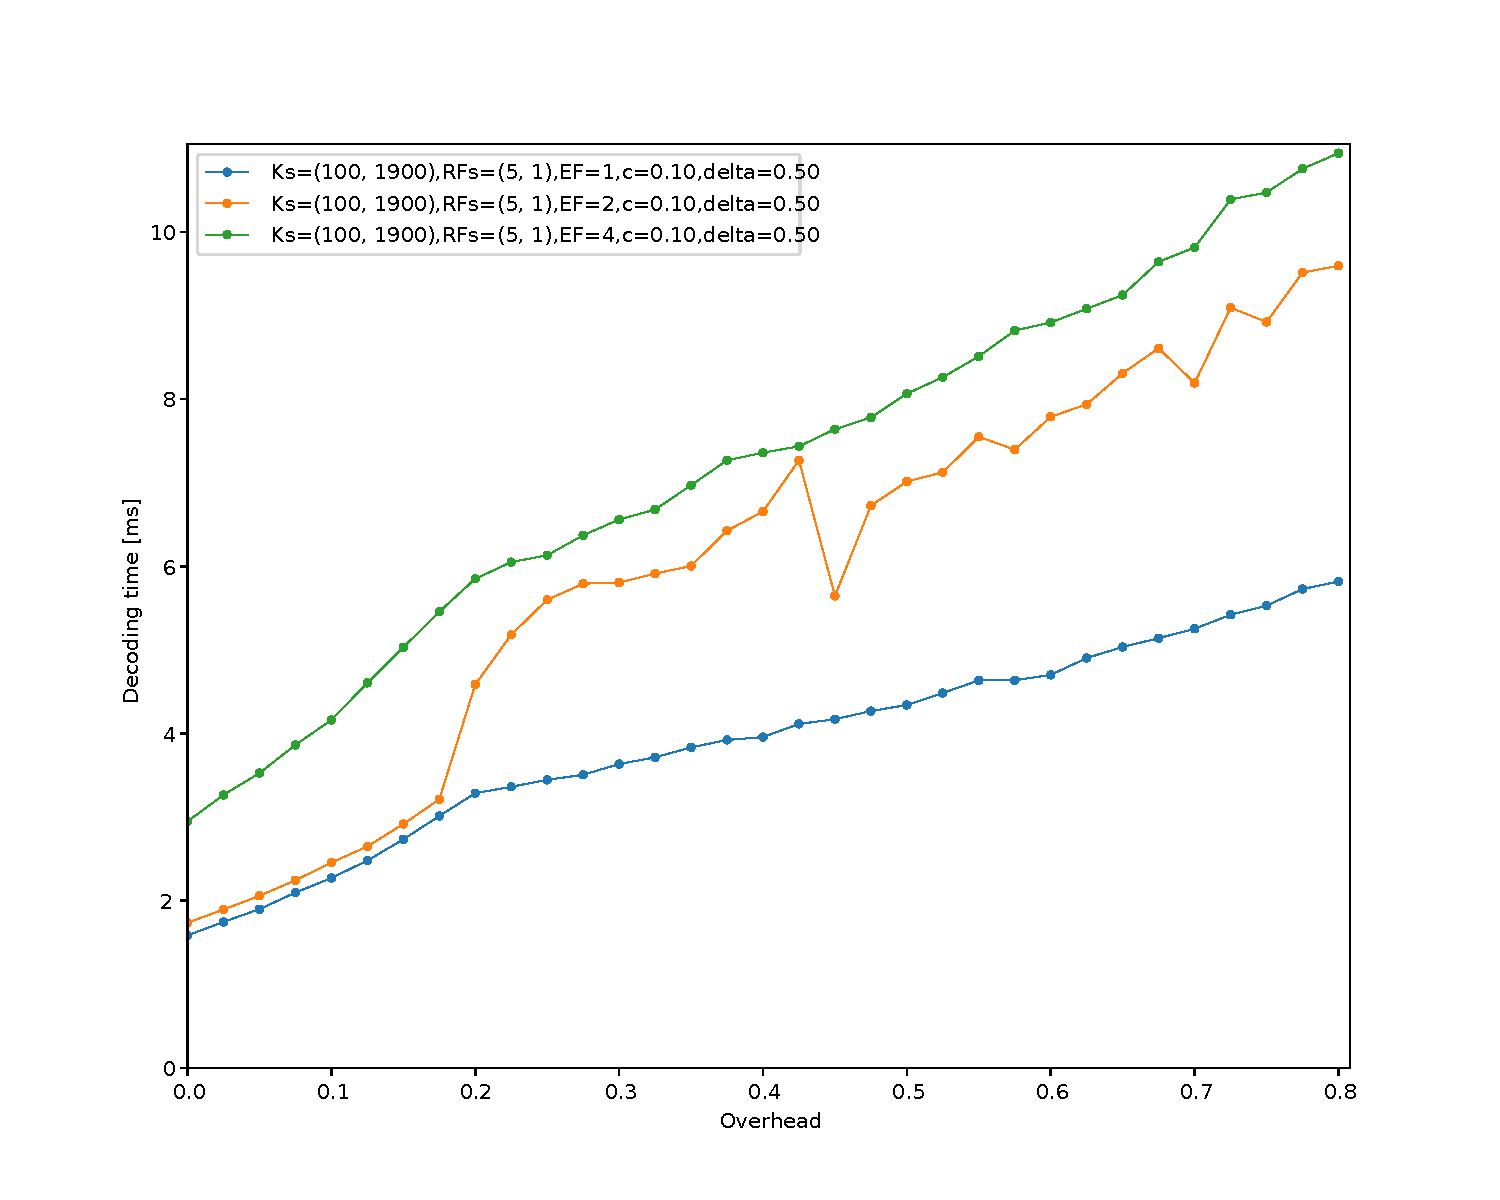
\includegraphics[width=\textwidth]{plot_dec_time_uep}
    \caption{Decodifica UEP}
    \label{fig:dectime_uep}
  \end{subfigure}
  \caption{Tempi medi di codifica e decodifica per un blocco di
    $K=2000$ pacchetti codificato usando EEP o UEP ($K_0 = 100$,
    $RF_0=5$) con $EF \in \{1,2,4,8,16\}$.}
  \label{fig:encdec}
\end{figure}
%
Si può vedere che l'andamento è coerente con \cite{uep}: entrambi i
tempi di codifica aumentano linearmente al crescere del'overhead e
sub-linearmente al crescere del fattore di espansione; i tempi di
decodifica crescono velocemente, in entrambi i casi, fino a un livello
di overhead in cui quasi tutti i pacchetti sono decodificabili e, in
seguito, la crescita diventa lineare e molto più lenta.
%
Confrontando le figure~\ref{fig:dectime_eep} e~\ref{fig:dectime_uep}
si vede che, per overhead bassi, l'uso dell'UEP aumenta molto i tempi
di decodifica, ma tende ad assestarsi su valori simili al caso EEP una
volta raggiunto un overhead tale da decodificare quasi tutti i
pacchetti.

I valori dei tempi di decodifica trovati in questa tesina sono dello
stesso ordine di grandezza di quelli riportati in \cite{uep}, invece i
tempi di codifica (figure~\ref{fig:enctime_eep}
e~\ref{fig:enctime_uep}) sono molto più alti, sia confrontandoli con i
grafici dell'articolo che coi tempi per la decodifica sullo stesso
computer.
%
Questo può essere spiegato dal fatto che, mentre l'implementazione del
message passing usata nelle simulazioni è scritta in C++, la
generazione dei vettori di codifica è effettuata da uno script più
lento scritto in Python.

\subsection{Scelta della dimensione dei pacchetti}
\label{sec:pktsize}
Il paper \cite{uep} considera simboli di 1 byte durante la codifica,
ma questa scelta non è praticabile nel caso si vogliano effettivamente
trasmettere dei pacchetti codificati.
%
Il motivo è dato dall'overhead introdotto aggiungendo degli header di
dimensione fissa di 15 byte a ogni pacchetto, infatti avere pacchetti
di lunghezza $L=1$ comporterebbe un overhead del 1500 \% dovuto solo
agli header.

Questo overhead decresce all'aumentare della dimensione dei pacchetti
$L$, tuttavia bisogna considerare anche l'overhead introdotto dalla
segmentazione del video H264, che non sarebbe presente nel caso $L=1$.
%
%% Il video H264 è composto da pacchetti (detti NALU) di dimensioni
%% variabili che devono essere aggregati o segmentati in pacchetti di
%% dimensione fissa $L$.
%
Il fatto di considerare due diverse classi di priorità per le NALU
richiede di inserire un certo numero di byte di padding ogni volta che
termina una sequenza consecutiva di NALU con la stessa priorità, per
ottenere un numero intero di pacchetti di lunghezza $L$.

Tenendo conto di entrambi questi contributi all'overhead per il video
usato in \cite{uep}, si ottiene il grafico mostrato in
figura~\ref{fig:pktsize} ed è possibile individuare il valore $L =
388$ che minimizza l'overhead introdotto prima di incapsulare i
pacchetti in UDP.
% Best packet size = 388
% Min overhead = 0.069367
% With UDP+IP:
% Best packet size = 671
% Min overhead = 0.123669
\begin{figure}[H]
  \centering
  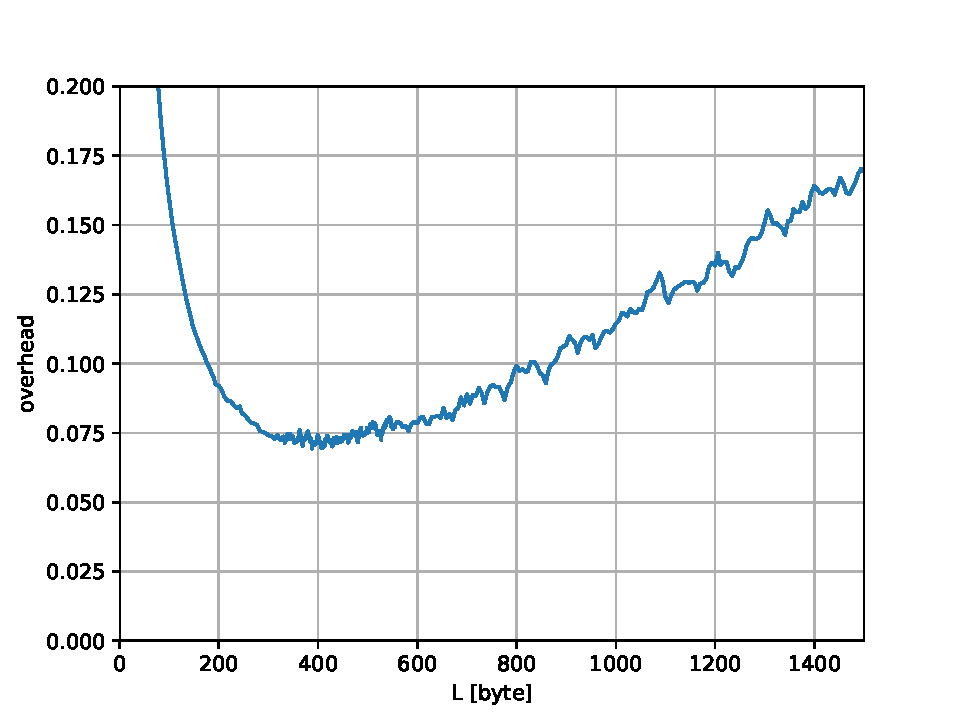
\includegraphics[width=0.8\textwidth]{plot_overhead}
  \caption{Overhead introdotto prima del livello UDP, al variare della
    dimensione $L$ dei pacchetti.}
  \label{fig:pktsize}
\end{figure}

\subsection{Simulazione del sistema completo}
Come scritto nel paragrafo~\ref{sec:complications}, l'esecuzione
del sistema completo è molto onerosa in termini di tempo, quindi in
questa tesina è stato preferito fornire dei grafici più precisi
simulando solamente il message passing.
%
L'esecuzione del sistema completo comunque fornisce risultati coerenti
con le simulazioni dei paragrafi precedenti, come è possibile vedere
in figura~\ref{fig:iid_real}.
%
Ripetendo lo stesso video usato in \cite{uep} fino a ottenere 4050
frame, usando pacchetti della dimensione ottimale trovata nel
paragrafo~\ref{sec:pktsize} e gli stessi parametri del
paragrafo~\ref{sec:iid} sono state ottenute le PER mostrate nella
figura~\ref{fig:iid_real}.
%
\begin{figure}[H]
  \centering
  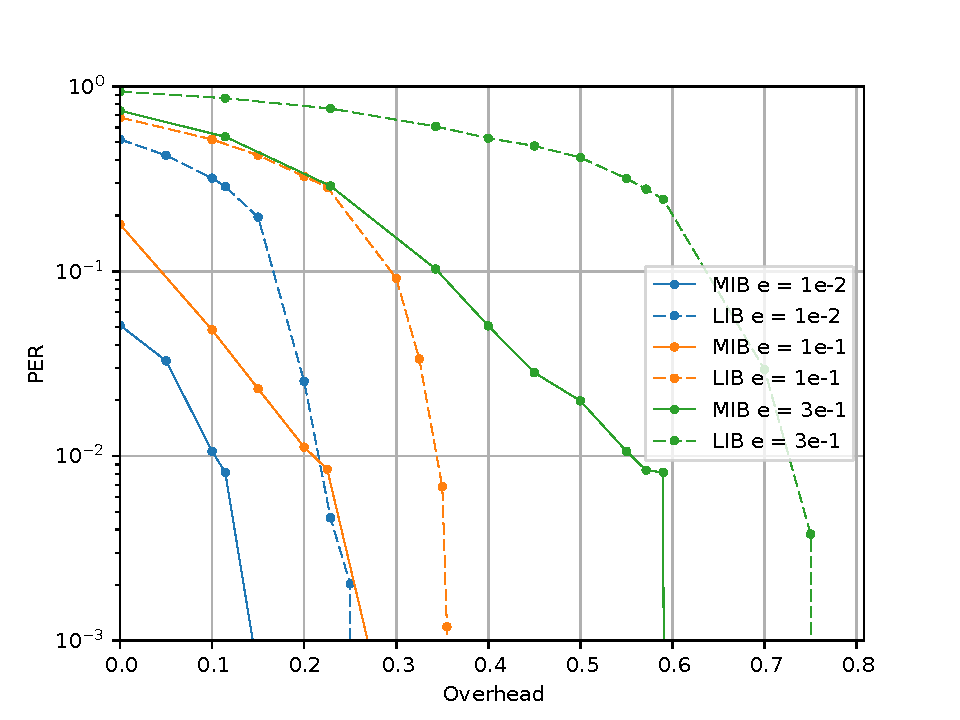
\includegraphics[width=0.8\textwidth]{plot_iid_real}
  \caption{Packet error rate ottenuta dal sistema completo al variare
    dell'overhead.}
  \label{fig:iid_real}
\end{figure}
%
Il canale è stato simualato scartando pacchetti UDP al client con una
data probabilità $e$, in modo simile alle simulazioni precedenti,
avendo sia il client che il server in esecuzione sullo stesso
computer.
%
Per permettere un confronto con i risultati delle simulazioni, è stato
tenuto conto solo dell'overhead introdotto dalla codifica dei
pacchetti segmentati, ignorando il contributo del padding e degli
header.

\section{Conclusioni} % Max 0.5 pages
%In conclusione, riassumendo, le diverse componenti del progetto sono
%\begin{itemize}
%\item Libreria JSVM per la codifica e decodifica di flussi video non compressi (C++)\\
%Classe per la lettura e la scrittura di pacchetti NAL
%\item Server e client TCP (C++)\\
%Utilizzo della libreria Protocol Buffers di Google per il passaggio dei parametri necessari alla libreria H.264
%\item Server e client UDP (C++)
%\item Codificatore e decodificatore a fontana (C++ e Python)
%\item Codificatore per protezione non uniforme (C++ e Python)
%\item Classe per l'algoritmo di message passing (C++ e Python)
%\item Logger (C++ e Python)
%\item Modelli del canale (senza errori, con errori i.i.d. e con errori correlati) (C++ e Python)
%\item Analisi dei dati e grafici dei risultati (Python)
%\end{itemize}
Per quanto riguarda il canale privo di errori, l'obbiettivo di implementare e testare l'algoritmo per la codifica UEP è stato raggiunto e i dati ottenuti sono compatibili con i dati 
presentati nel paper \cite{uep}.
%Le performance dell'algoritmo sono migliorabili da un punto di vista di complessità di calcolo,
%in quanto confrontando i risultati ottenuti in figura \ref{fig:encdec} con \cite{uep} si nota
%che la pendenza della curva tempo di codifica / decodifica contro overhead sia maggiore
%per la nostra realizzazione dell'algoritmo.\\
Il canale con errori i.i.d. può essere utilizzato, imponendo una
Packet Error Rate a livello applicazione bassa a piacere, semplicemente variando la quantità di ridondanza aggiunta.
Come si vede in figura \ref{fig:iid_oh}, anche per un canale con probabilità d'errore
 $P_e = 0.3$, la PER è inferiore a $10^{-8}$ imponendo un overhead contenuto.\\
Dalla stessa figura si nota come al variare della probabilità di 
errore del canale, la curva PER vs overhead sia traslata rispetto all'overhead; ciò dimostra
che se la PER del canale varia, la PER a livello applicazione può essere contenuta
variando l'overhead.\\
Nell'eventualità in cui il canale presenti errori correlati,
la possibilità di aumentare la lunghezza del blocco di pacchetti codificati oltre la lunghezza media della sequenza
di slot cattivi consecutivi può essere utile ad abbassare la PER anche senza aumentare l'overhead aggiunto.\\
Se non è possibile aumentare la dimensione del blocco oltre la lunghezza media $\EnB$, è bene 
tener presente che la quantità di overhead aggiunto ad ogni blocco può essere comunque
regolata in base a stime della condizione del canale, in modo da soddisfare eventuali condizioni
sulla probabilità d'errore a livello applicazione.\\
Se ci sono vincoli sulla dimensione massima del blocco, che possono derivare 
da vincoli sul delay massimo nella ricezione dei pacchetti, è utile mantenere 
piccola la dimensione del blocco e sfruttare l'algoritmo di protezione non uniforme, infatti,
per i canali testati ($\pi_B \in\{10^{-1},10^{-2}\}$), dalle figure \ref{fig:markov_pi100small} 
e \ref{fig:markov_pi10small} si evince come quando i blocchi 
in uscita dall'encoder abbiano dimensioni inferiori a $K^* \approx 2100$ pacchetti, 
la protezione non uniforme abbia prestazioni migliori della protezione uniforme sia per quanto riguarda la
parte MIB che per quanto riguarda la parte LIB.\\
Per blocchi di dimensione maggiore, l'algoritmo EEP ha prestazioni 
migliori rispetto alle prestazioni dell'algoritmo UEP, in quanto la Packet
Error Rate del caso EEP è inferiore al caso UEP (sia MIB che LIB) quando la dimensione del blocco aumenta.\\
In conclusione, sia per canali con errori indipendenti che per canali con errori correlati, l'algoritmo di protezione basato su UEP testato in questa tesina è utile ed efficiente. Durante l'implementazione è stato possibile imparare come scrivere un software che applichi una codifica e trasmetta realmente dei pacchetti attraverso i socket e valutarne le prestazioni.
%\begin{figure}[H]
%	\makebox[\textwidth][c]{\includegraphics[width=16cm]{G10labE_f3.eps}}
%	\caption{Componenti di $\hat{s}$}\label{fig:s2}
%\end{figure}

% Between 3-15 refs
\printbibliography[heading=bibnumbered, title=Bibliografia]
\end{document}
